% Build note:
% Compile from docs/ with: latexmk -pdf report.tex
% Aux files go to docs/.latex_aux via docs/.latexmkrc.
\documentclass[conference]{IEEEtran}
\IEEEoverridecommandlockouts
% The preceding line is only needed to identify funding in the first footnote. If that is unneeded, please comment it out.
\usepackage{cite}
\usepackage{amsmath,amssymb,amsfonts}
\usepackage{algorithmic}
\usepackage{booktabs}
\usepackage{graphicx}
\usepackage{dblfloatfix}
\usepackage{placeins}
\usepackage{textcomp}
\usepackage{xcolor}
\raggedbottom
\setcounter{topnumber}{4}
\setcounter{bottomnumber}{4}
\setcounter{totalnumber}{8}
\renewcommand{\topfraction}{0.95}
\renewcommand{\bottomfraction}{0.95}
\renewcommand{\textfraction}{0.05}
\renewcommand{\floatpagefraction}{0.85}
\setlength{\textfloatsep}{8pt plus 2pt minus 2pt}
\setlength{\floatsep}{8pt plus 2pt minus 2pt}
\setlength{\intextsep}{8pt plus 2pt minus 2pt}
\setlength{\abovecaptionskip}{4pt}
\setlength{\belowcaptionskip}{0pt}
\def\BibTeX{{\rm B\kern-.05em{\sc i\kern-.025em b}\kern-.08em
    T\kern-.1667em\lower.7ex\hbox{E}\kern-.125emX}}
\begin{document}

\title{Parallel Performance Analysis of Ant Colony Optimization with OpenMP, MPI, and Hybrid Domain Decomposition}

\author{\IEEEauthorblockN{1\textsuperscript{st} Given Name Surname}
\IEEEauthorblockA{\textit{dept. name of organization (of Aff.)} \\
\textit{name of organization (of Aff.)}\\
City, Country \\
email address or ORCID}
\and
\IEEEauthorblockN{2\textsuperscript{nd} Given Name Surname}
\IEEEauthorblockA{\textit{dept. name of organization (of Aff.)} \\
\textit{name of organization (of Aff.)}\\
City, Country \\
email address or ORCID}
\and
\IEEEauthorblockN{3\textsuperscript{rd} Given Name Surname}
\IEEEauthorblockA{\textit{dept. name of organization (of Aff.)} \\
\textit{name of organization (of Aff.)}\\
City, Country \\
email address or ORCID}
\and
\IEEEauthorblockN{4\textsuperscript{th} Given Name Surname}
\IEEEauthorblockA{\textit{dept. name of organization (of Aff.)} \\
\textit{name of organization (of Aff.)}\\
City, Country \\
email address or ORCID}
\and
\IEEEauthorblockN{5\textsuperscript{th} Given Name Surname}
\IEEEauthorblockA{\textit{dept. name of organization (of Aff.)} \\
\textit{name of organization (of Aff.)}\\
City, Country \\
email address or ORCID}
\and
\IEEEauthorblockN{6\textsuperscript{th} Given Name Surname}
\IEEEauthorblockA{\textit{dept. name of organization (of Aff.)} \\
\textit{name of organization (of Aff.)}\\
City, Country \\
email address or ORCID}
}

\maketitle

\begin{abstract}
This document analyzes the parallel execution of an Ant Colony Optimization simulation over a fractal terrain. The study compares a shared-memory OpenMP implementation, a distributed-memory MPI implementation based on subdomain decomposition with halo exchange and ant migration, and a hybrid MPI+OpenMP variant that introduces intra-subdomain thread-level parallelism. The reported results focus on iteration time, computation time, rendering cost, and communication overhead across multiple colony sizes in order to identify the practical scalability limits of each model and the tradeoffs between computation and communication.
\end{abstract}

\begin{IEEEkeywords}
ant colony optimization, parallel computing, OpenMP, MPI, hybrid programming, domain decomposition
\end{IEEEkeywords}

\section{Introduction}
The Ant Colony Optimization problem is one of the most widely studied metaheuristics for the simulation of collective behaviors in nature. The implementation of the algorithm is proposed from the definition of multiple artificial ants, either as a class or from the vector-based description of their properties. Each of these artificial entities makes movement decisions based on a combination of local heuristic information and a shared collective memory, usually modeled through an artificial pheromone. This optimization approach was introduced by Marco Dorigo in the 1990s \cite{Dorigo}.

The importance of this optimization lies in its ability to address problems in which the search space grows rapidly and where exact methods face difficulties in terms of computational scalability. Nevertheless, in large-scale scenarios, not only because of the size of the ant colony but also due to the complexity of the map, limitations may arise in computation times and in the efficient handling of increasingly larger scales.

In this context, the imminent need emerges to incorporate scalability and parallelization strategies for ACO, aimed at reducing the execution time of each algorithm by decreasing the computational load and facilitating the treatment of even larger entities. For this reason, the present document addresses parallelization with shared memory through OpenMP, as well as two different distributed-memory parallelization strategies using MPI, with the objective of improving the handling of large instances in the description of the collective behavior of ants.

\subsection{Simulation times measurement
}
The measured times are defined so as to separate the simulation into clearly differentiated phases, which makes it possible to identify the contribution of each operation to the overall computational cost. In \texttt{event\_poll} (see Table~\ref{tab:timing_summary}), the time spent handling SDL events is recorded, including window closing, basic interaction, and event-queue updates; this corresponds to interface overhead rather than algorithmic work.

In \texttt{ants\_advance} (Table~\ref{tab:timing_summary}), the behavioral core of the ants is measured, including movement decisions, neighboring pheromone reads, food transport, collection accounting, and pheromone marking. In \texttt{evaporation} (Table~\ref{tab:timing_summary}), only the pheromone evaporation stage is measured, which is characterized by ordered memory traversal and conditional evaporation logic and is therefore favorable for locality- and vectorization-based optimization. In \texttt{update} (Table~\ref{tab:timing_summary}), the consolidation of the pheromone state at the end of the step is included, together with buffer exchanges, restoration of special cells, reimposition of nest and food sources, and map maintenance. Finally, \texttt{advance\_total} (Table~\ref{tab:timing_summary}) provides the most representative measure of the simulation core cost because it integrates \texttt{ants\_advance}, \texttt{evaporation}, and \texttt{update}.

In \texttt{render} (Table~\ref{tab:timing_summary}), the time required to draw the scene is measured, including the \texttt{blit} stage and the full screen-frame representation cost. All these contributions are ultimately included in \texttt{iteration\_total} (Table~\ref{tab:timing_summary}), which represents the complete cost of one simulation iteration.

Additionally, general simulation information is stored, including the number of measured iterations, the final amount of food after the simulation ends, and the iteration at which the first food unit arrives.

As a concrete reference, Table~\ref{tab:timing_summary_threads1_ants5000} summarizes the measured values obtained from the non-vectorized implementation for a simulation of 5000 ants executed until the first food unit reaches the nest and during the 10 subsequent iterations. In this sense, the average, minimum, and maximum values reported in the table correspond to per-iteration results.

\begin{table}[htbp]
\centering
\caption{Summary of measured execution times in the simulation.}
\label{tab:timing_summary}
\begin{tabular}{p{0.24\linewidth} p{0.68\linewidth}}
\hline
\textbf{Time metric} & \textbf{Brief description} \\
\hline
\texttt{event\_poll} & SDL event handling. \\
\texttt{ants\_advance} & Ant movement and decisions. \\
\texttt{evaporation} & Pheromone evaporation. \\
\texttt{update} & State consolidation and restoration. \\
\texttt{advance\_total} & Total simulation-core cost. \\
\texttt{render} & Frame rendering time. \\
\texttt{iteration\_total} & Total iteration time. \\
\hline
\end{tabular}
\end{table}

\begin{table}[!htbp]
\centering
\caption{Measured timing statistics for the non-vectorized implementation with 1 thread and 5000 ants.}
\label{tab:timing_summary_threads1_ants5000}
\scriptsize
\setlength{\tabcolsep}{2.8pt}
\renewcommand{\arraystretch}{1.08}
\resizebox{\columnwidth}{!}{%
\begin{tabular}{lrrrrr}
\toprule
\textbf{Metric} & \textbf{Count} & \textbf{Total [ms]} & \textbf{Mean [ms]} & \textbf{Min [ms]} & \textbf{Max [ms]} \\
\midrule
\texttt{event\_poll} & 2572 & 54.651 & 0.021 & 0.007 & 0.938 \\
\texttt{ants\_advance} & 2572 & 4099.533 & 1.594 & 1.136 & 4.595 \\
\texttt{evaporation} & 2572 & 922.001 & 0.358 & 0.255 & 0.956 \\
\texttt{update} & 2572 & 8.828 & 0.003 & 0.002 & 0.054 \\
\texttt{advance\_total} & 2572 & 5030.363 & 1.956 & 1.416 & 5.272 \\
\texttt{render} & 2572 & 34364.856 & 13.361 & 2.466 & 34.371 \\
\texttt{blit} & 2572 & 39733.913 & 15.449 & 0.457 & 16.907 \\
\texttt{iteration\_total} & 2572 & 79184.842 & 30.787 & 15.232 & 48.037 \\
\bottomrule
\end{tabular}%
}
\par\vspace{2pt}\parbox{\columnwidth}{\raggedright\footnotesize\textit{Note.} Additional run metadata: \texttt{total\_iterations}=2572, \texttt{measured\_iterations}=2572, \texttt{final\_food\_quantity}=1, and \texttt{first\_food\_iteration}=2562.}
\end{table}

It becomes evident from the results of the process that the dominant component within each of the iterations of the ant dynamics is rendering, whereas within the specific computation stages only the advance of the ants is the one that represents the largest average time within each of the iterations of the process. It is also observed that this behavior is not limited to the drawing stage alone, since the associated \texttt{blit} cost also occupies a significant fraction of the full iteration time, which reinforces that the rendering pipeline dominates the global execution budget, while within the simulation core the greatest impact is concentrated in \texttt{ants\_advance}.

\subsection{Algorithmic Equivalence}
A general methodology is proposed for the analysis of the general behavior of the parallelization strategies that are proposed to be implemented within the methodological framework of the stated problem. In the first place, a generalized execution and comparison framework is proposed, corresponding to the execution of the algorithm until the first food item reaches the nest and the 10 subsequent iterations. In this context, it is intended that the results provided by all the algorithms make it possible to identify the number of iterations at which this milestone is reached in the simulation, with the idea of verifying that this number is the same for ant colonies of the same size and, in this way, verifying that the simulated dynamics are in fact equivalent and therefore that their results are comparable.

It is also proposed to record the amount of food that reaches the nest during those 10 subsequent iterations as a sample of equivalence in the dynamics of the colony after the arrival of the first food item. Under this criterion, the common observation window is not defined only by a fixed number of iterations, but by a shared behavioral event in the simulation, which makes it possible to compare the different implementations from an equivalent point in the evolution of the colony. In this way, the comparison framework is intended not only to contrast execution times, but also to verify that the underlying simulated behavior remains consistent across the different parallelization strategies.

\section{Distributed subdomain mpi}

In this section, the implementation of an optimization strategy over the fractal domain is proposed based on the decomposition of the terrain into two-dimensional subdomains, which are managed by each MPI process. Each one is responsible for managing one of these subdomains in the map, considering the boundary effects between two-dimensional subdomains through the concept of ghost cells. Additionally, only the logic for generating a global terrain is preserved in the root node for data collection and subsequent rendering.

The domain decomposition is constructed through a 2D MPI Cartesian topology. For this, \texttt{MPI\_Dims\_create} is used for the automatic factorization of the processes into a two-dimensional mesh of dimensions. Then, Cartesian communicators are created for the direct neighbors in the four directions: up, down, left, and right. In this way, each of the processes knows its Cartesian coordinates associated with the fractal terrain, as well as its local size and offset in both directions.

In addition to the interior block, each of the processes preserves a ghost-cell crown of thickness determined by parameterization in the case of the simulation, which is taken into account for local storage in the stride variables. The memory linear accesses as well as the indexations are performed considering the effect of those ghost cells that are implemented for the management of the neighborhood of the subdomains and the boundary conditions. It is this ghost-cell structure that makes it possible for MPI communication not to be required for each one of the ants that is located at the edge or boundary of its subdomain, considering that the algorithm only needs the immediate neighbors at a single-cell distance; therefore, a single layer of thickness 1 is sufficient to satisfy the algorithmic requirement.

The exchange of ghost cells for the fields that are static during the simulation, as in the case of the terrain and the cell type, is carried out with a classical one-halo-layer-per-boundary policy. Each process packs its first and last interior row for up/down, and its first and last interior column for left/right; then it launches non-blocking \texttt{MPI\_Irecv} and \texttt{MPI\_Isend} with the corresponding neighbors.


\subsection{Pheromone system}
The pheromone system is organized into two channels, each of which has its own memory buffer, which allows the distinction of two trails with a different semantics: an ant without load consults channel 0, while a loaded ant consults channel 1. To avoid coherence problems between the current pheromone state and the next one, two copies are preserved, one current and one next, so that all ants read the current version but write to the next version, and at the end of the step the exchange or swap is performed.

In terms of the exchange, instead of sending \texttt{v1} and \texttt{v2} separately between the subdomains, what is done is to pack them into a single interleaved buffer, for each one of the cells at the boundary of the subdomains. This provides a reduction in the number of messages to be sent with respect to independent fields, mainly because the communication costs exceed the cache-query costs associated with the buffer.




\subsection{Ant migration}


When an ant, as part of its movement, crosses a boundary and therefore the destination cell no longer belongs to the process to which this ant is assigned, a \texttt{TransitAnt} is constructed that contains the information associated with the properties of the ant, including the information for the pheromone update in the cell into which the ant enters before migration. The migration protocol is implemented with two neighborhood collectives over the Cartesian communicator. First, each process exchanges with its four neighbors the counts of outgoing ants per direction (up/down/left/right) by using \texttt{MPI\_Neighbor\_alltoall}. Then, with the received counts, it exchanges the payload arrays through \texttt{MPI\_Neighbor\_alltoallv} with \texttt{MPI\_BYTE}, transmitting contiguous blocks of \texttt{TransitAnt} with size \texttt{count * sizeof(TransitAnt)}.

Finally, it concatenates what is received into an \texttt{active} vector. The ants that arrive at the process do not mean that they have already completed their step; that is why it calls \texttt{process\_single\_ant(...)} on each received active ant. That function continues the movement from the partial state of the ant; and if during that continuation it crosses another boundary again, it sends it again to another neighbor. The loop is not exited until the entire system remains ``at rest'' with respect to migrations, that is, until there is no ant pending to complete its distributed step. The global active-ant total is computed with \texttt{MPI\_Iallreduce(..., MPI\_SUM, ...)} and checked periodically (not every migration round), reducing global synchronization frequency while preserving the same completion criterion (\texttt{global\_active == 0}).


\subsection{Time measurement}

Given the particular conditions of the fractal-terrain partitioning and the ownership of ants over two-dimensional subdomains, it is necessary to add new timing measurements in order to identify the computational costs of the strategies implemented for parallelization with distributed memory. The time \texttt{mpi\_halo\_exchange} is included to measure the time taken by the halo exchange of pheromones in each iteration, which accounts for the communication time associated with the fixed neighborhood imposed by the spatial decomposition.

\texttt{mpi\_migration} measures the time spent within \texttt{advance} in the exchange of ants between one rank and another, and is therefore responsible for measuring the cost associated with the distribution of the ant population across the subdomains handled by the processes. For its part, the variable \texttt{mpi\_food\_allreduce} accounts for the blocking wait time associated with the non-blocking global food reduction (\texttt{MPI\_Iallreduce + MPI\_Wait}), after overlapping part of that communication with local computation.

\texttt{mpi\_render\_comm} measures \texttt{gather\_state\_for\_render(...)}, that is, the collection of the distributed state toward rank 0 in order to render pheromones and ants in a single global view. It is not the rendering itself, but rather the previous communication required for rendering. Finally, \texttt{halo\_ms\_local + migration\_ms\_local + food\_allreduce\_ms\_local + render\_comm\_ms\_local} are accumulated into \texttt{mpi\_total\_comm}, which accounts for the fraction of the total time spent in communication between MPI processes. Additionally, to reduce synchronization overhead in reporting, per-iteration timing reductions are aggregated and reduced in batches instead of reducing every metric in every iteration.

\begin{table}[htbp]
\centering
\caption{Additional MPI communication timing metrics.}
\label{tab:mpi_timing_summary}
\begin{tabular}{p{0.30\linewidth} p{0.58\linewidth}}
\hline
\textbf{Time metric} & \textbf{Brief description} \\
\hline
\texttt{mpi\_halo\_exchange} & Pheromone halo exchange. \\
\texttt{mpi\_migration} & Ant migration between ranks. \\
\texttt{mpi\_food\_allreduce} & Global food reduction. \\
\texttt{mpi\_render\_comm} & State gathering for rendering. \\
\texttt{mpi\_total\_comm} & Total MPI communication time. \\
\hline
\end{tabular}
\end{table}

\subsection{Results analysis}

It is therefore proposed to analyze the results of the MPI parallelization based on the subdivision into subdomains, and two elements become evident. The first is that the bottleneck in the execution of the simulations, both in the subdomain-based parallelization and in the other parallelization strategies that have been analyzed, lies in the graphical part of the algorithm as shown in Fig.~\ref{fig:mpi_total_breakdown_selected}. Even in the case in which the number of ants, and therefore the number of computational operations, grows up to 320000 ants in the colony, this causes the effect of the parallelization not to become necessarily evident in the analysis of the total time of each iteration in the simulation. However, if only the time consumed by the algorithm in \texttt{ant\_advance}, which corresponds to the total computation time of the algorithm, is analyzed, the dynamics differ considerably. In particular, the decomposition by components reveals that the computational stage preserves a favorable tendency with the increase in the number of processes, whereas the visual stage keeps a relatively high weight per iteration. This behavior explains why the global metric can suggest weak scaling even when the numerical core is effectively accelerated by the distributed scheme.

\begin{figure}[!htbp]
\centering
\begin{minipage}{0.48\columnwidth}
    \centering
    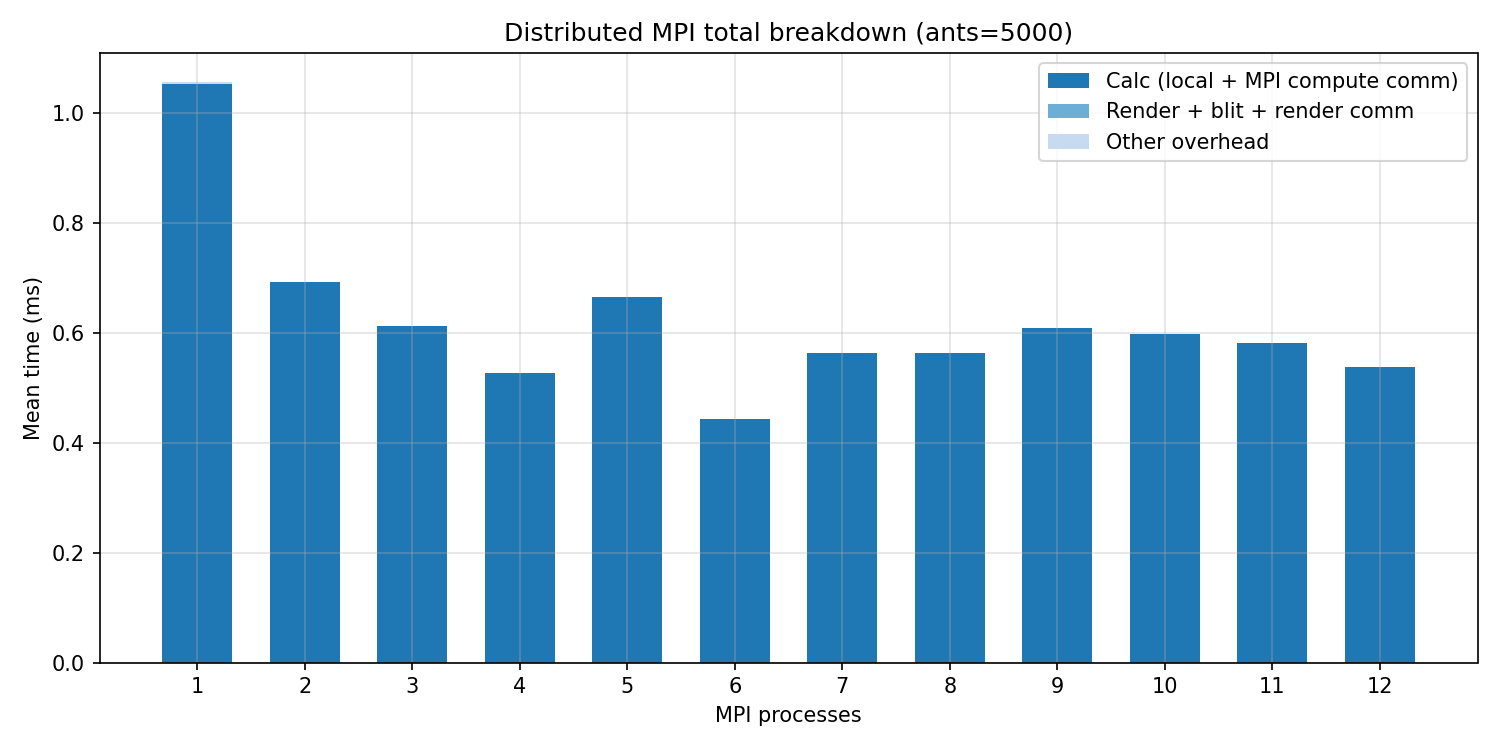
\includegraphics[width=\linewidth]{../distributed_subdomain_mpi/results/sweeps_render_food10/plots/mpi_total_breakdown_ants5000.png}
    \\[-2mm]
    {\footnotesize (a) 5000 ants}
\end{minipage}
\hfill
\begin{minipage}{0.48\columnwidth}
    \centering
    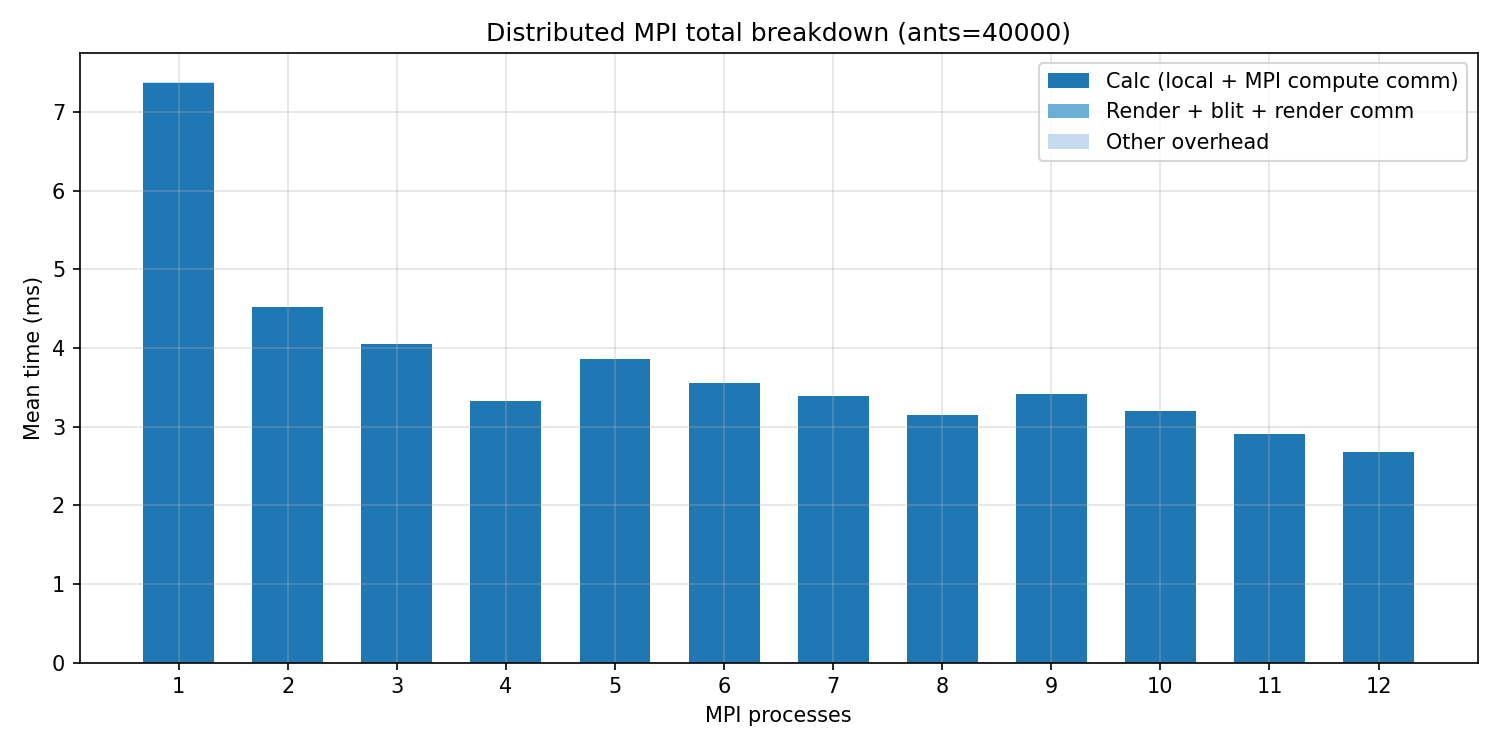
\includegraphics[width=\linewidth]{../distributed_subdomain_mpi/results/sweeps_render_food10/plots/mpi_total_breakdown_ants40000.png}
    \\[-2mm]
    {\footnotesize (b) 40000 ants}
\end{minipage}

\vspace{1mm}
\begin{minipage}{0.62\columnwidth}
    \centering
    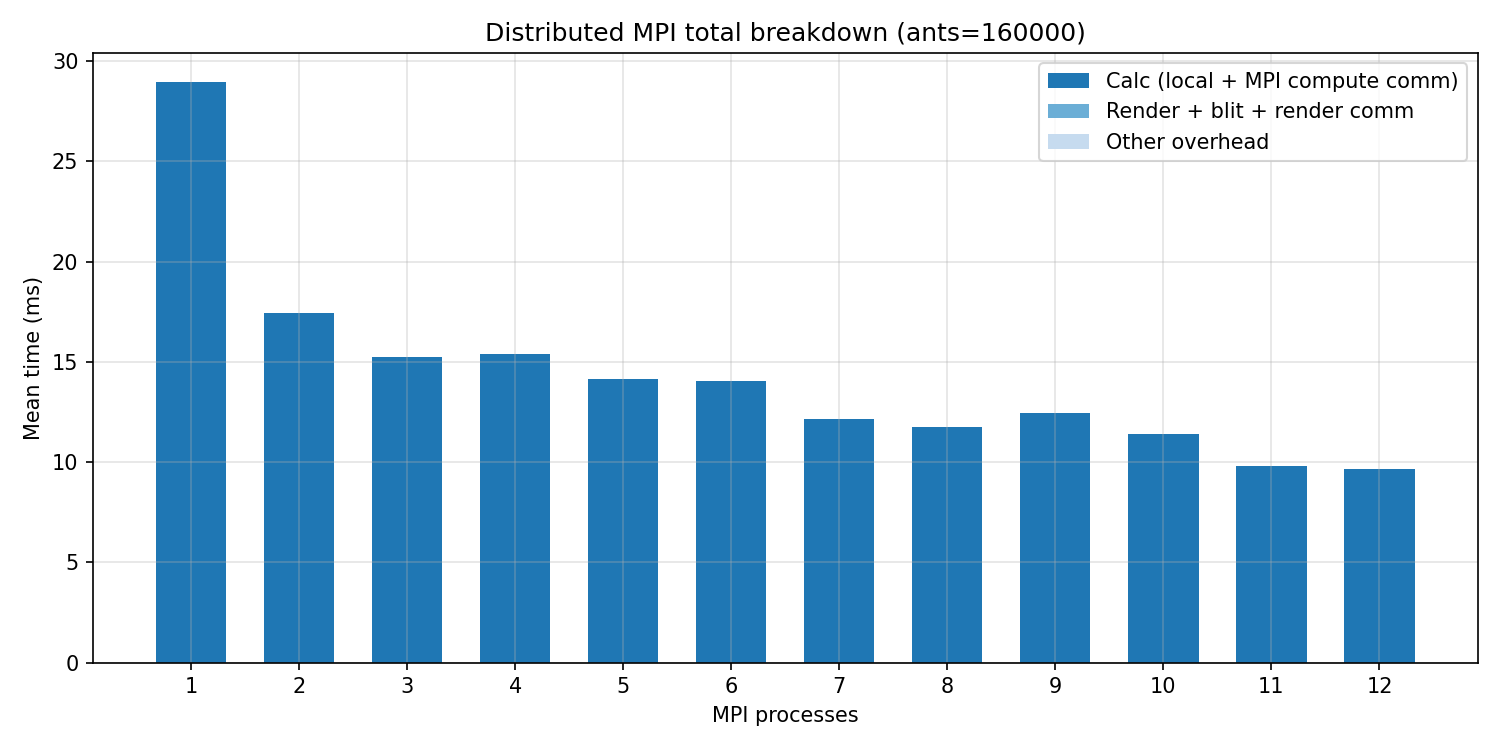
\includegraphics[width=\linewidth]{../distributed_subdomain_mpi/results/sweeps_render_food10/plots/mpi_total_breakdown_ants160000.png}
    \\[-2mm]
    {\footnotesize (c) 160000 ants}
\end{minipage}
\caption{MPI subdomain total iteration-time breakdown for selected colony sizes.}
\label{fig:mpi_total_breakdown_selected}
\end{figure}

When the number of ants is small, as in the case of a colony of 5000 ants, it is possible to observe the effect produced by the incorporation of more processes in the acceleration of the computation, reaching a maximum close to 2 when communications between processes are considered. Nevertheless, when the speedup without communication is considered, a much more marked growth effect can be seen, reaching a speedup greater than 3 for 12 processes. However, this difference between the real speedup of the computation and the speedup without considering communication becomes increasingly larger as more subdomains are added in the representation of the fractal terrain and the communication between processes increases as depicted in Fig.~\ref{fig:mpi_speedup_selected} and Fig.~\ref{fig:mpi_calc_only_selected}. The growth in the size of the ant colony leads to similar dynamics in terms of speedup, showing reductions as the number of ants increases and revealing behaviors in which, despite corresponding to a larger number of processes, the linearity of the executed actions or the cost of memory-access operations due to the growth of the buffers causes the resulting effect in terms of speedup to be somewhat smaller than in the case of a colony size of 5000 ants.

\begin{figure}[!htbp]
\centering
\begin{minipage}{0.48\columnwidth}
    \centering
    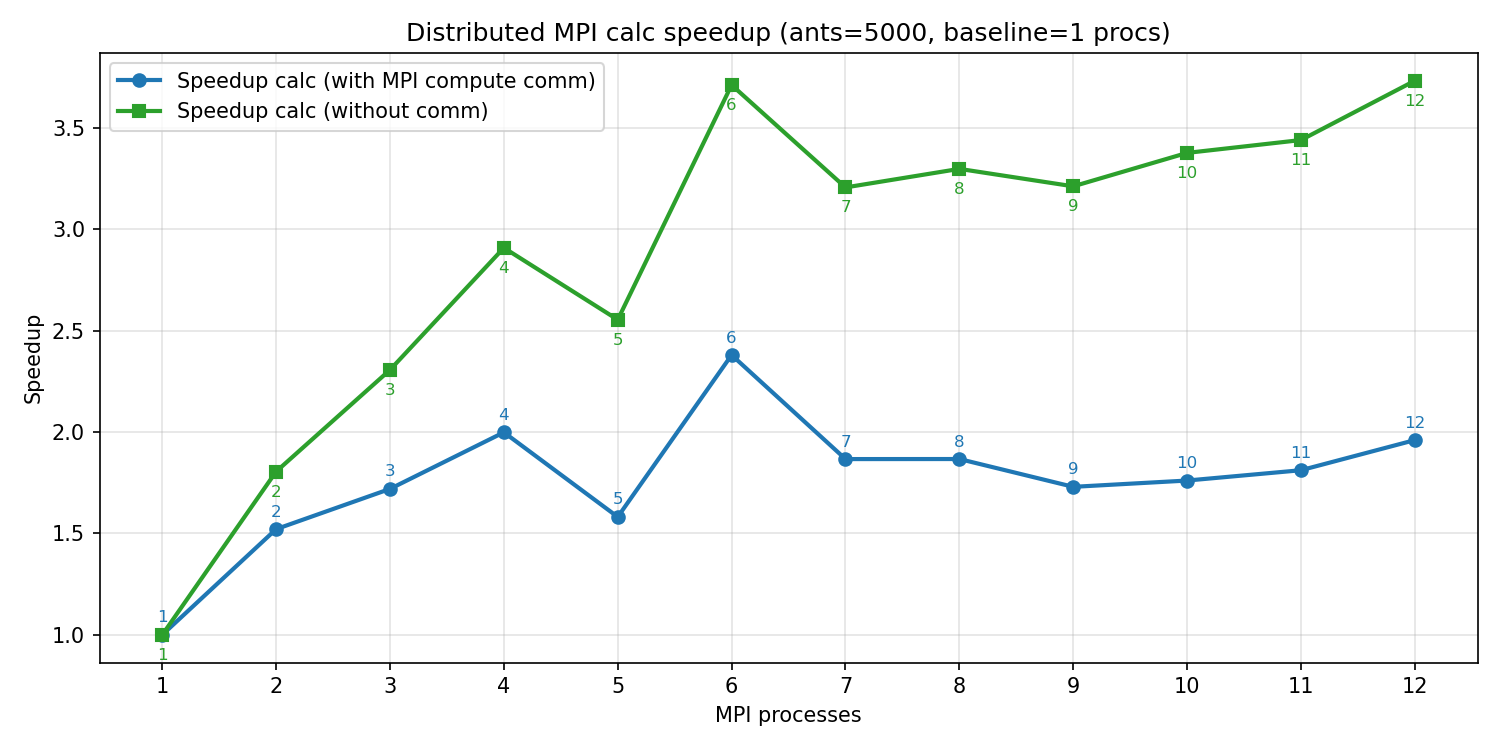
\includegraphics[width=\linewidth]{../distributed_subdomain_mpi/results/sweeps_render_food10/plots/mpi_calc_speedup_ants5000.png}
    \\[-2mm]
    {\footnotesize (a) 5000 ants}
\end{minipage}
\hfill
\begin{minipage}{0.48\columnwidth}
    \centering
    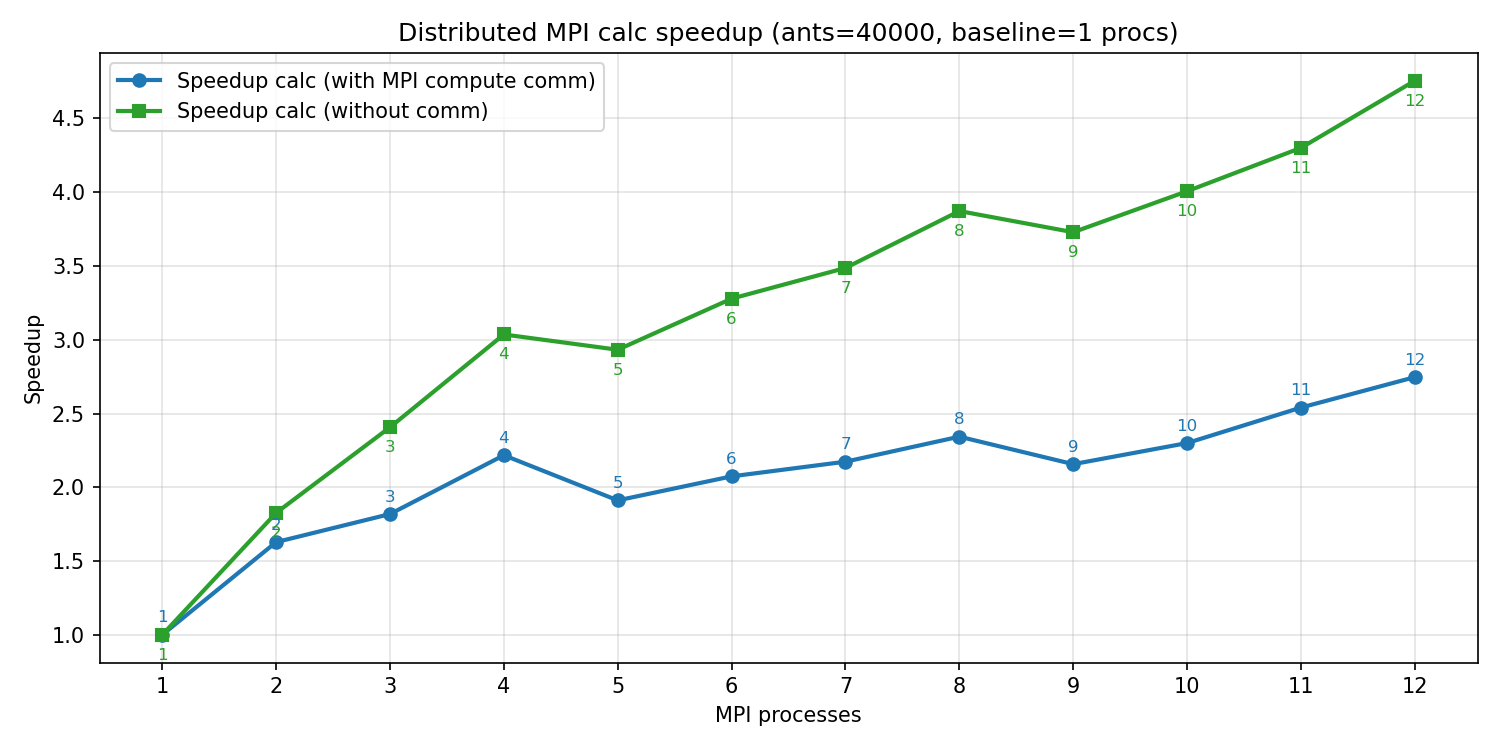
\includegraphics[width=\linewidth]{../distributed_subdomain_mpi/results/sweeps_render_food10/plots/mpi_calc_speedup_ants40000.png}
    \\[-2mm]
    {\footnotesize (b) 40000 ants}
\end{minipage}

\vspace{1mm}
\begin{minipage}{0.62\columnwidth}
    \centering
    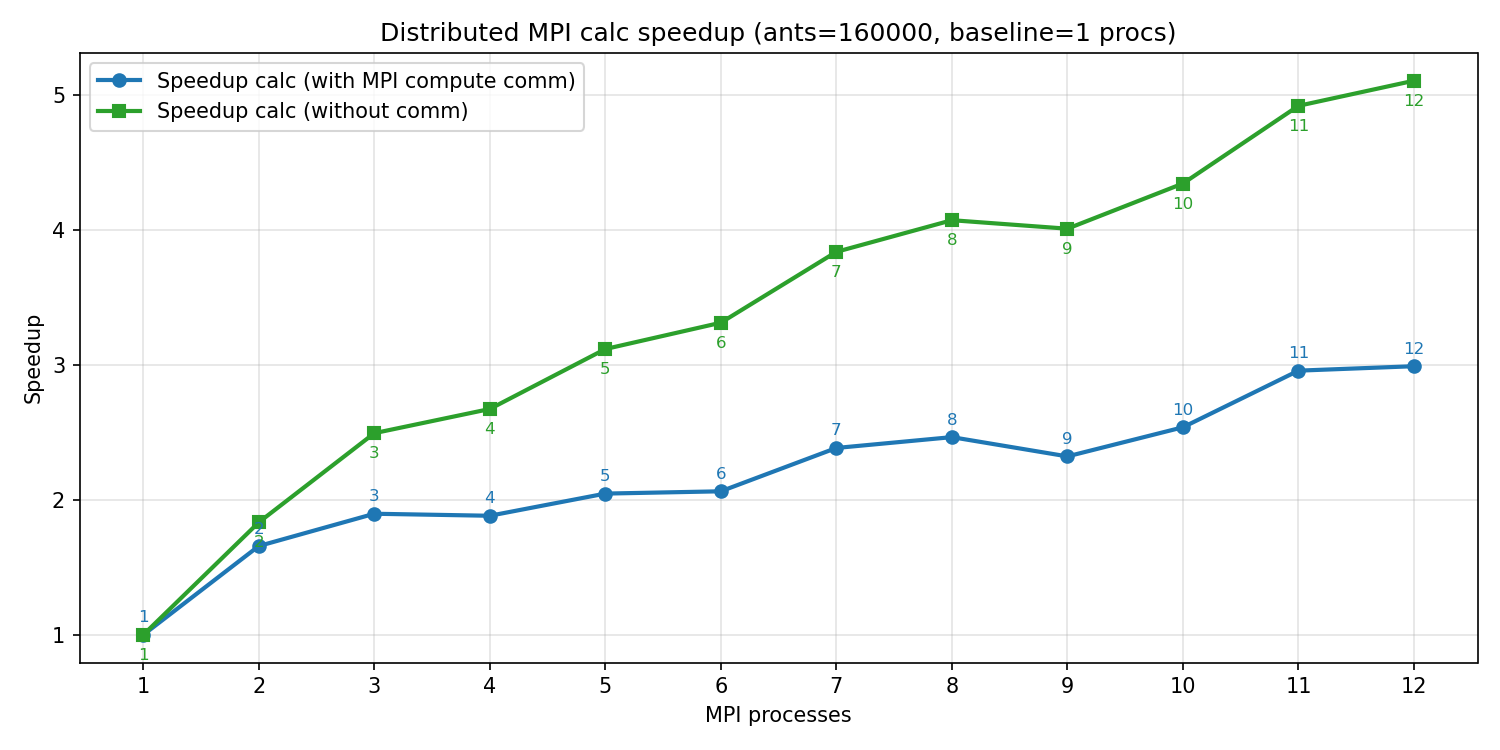
\includegraphics[width=\linewidth]{../distributed_subdomain_mpi/results/sweeps_render_food10/plots/mpi_calc_speedup_ants160000.png}
    \\[-2mm]
    {\footnotesize (c) 160000 ants}
\end{minipage}
\caption{MPI subdomain computation speedup (with and without communication) for selected colony sizes. The associated efficiency is computed with respect to compute MPI processes only, excluding rendering.}
\label{fig:mpi_speedup_selected}
\end{figure}

\begin{figure}[!htbp]
\centering
\begin{minipage}{0.48\columnwidth}
    \centering
    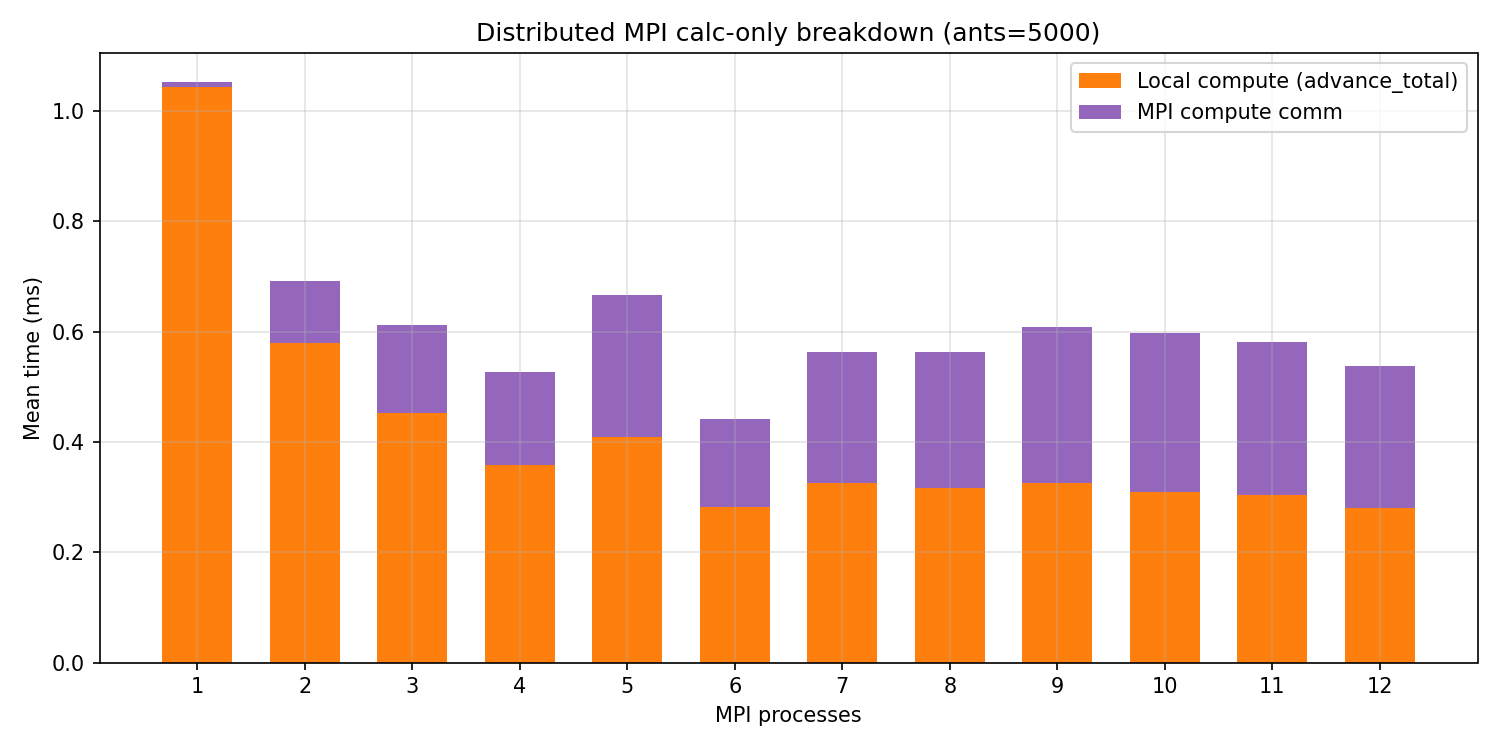
\includegraphics[width=\linewidth]{../distributed_subdomain_mpi/results/sweeps_render_food10/plots/mpi_calc_only_ants5000.png}
    \\[-2mm]
    {\footnotesize (a) 5000 ants}
\end{minipage}
\hfill
\begin{minipage}{0.48\columnwidth}
    \centering
    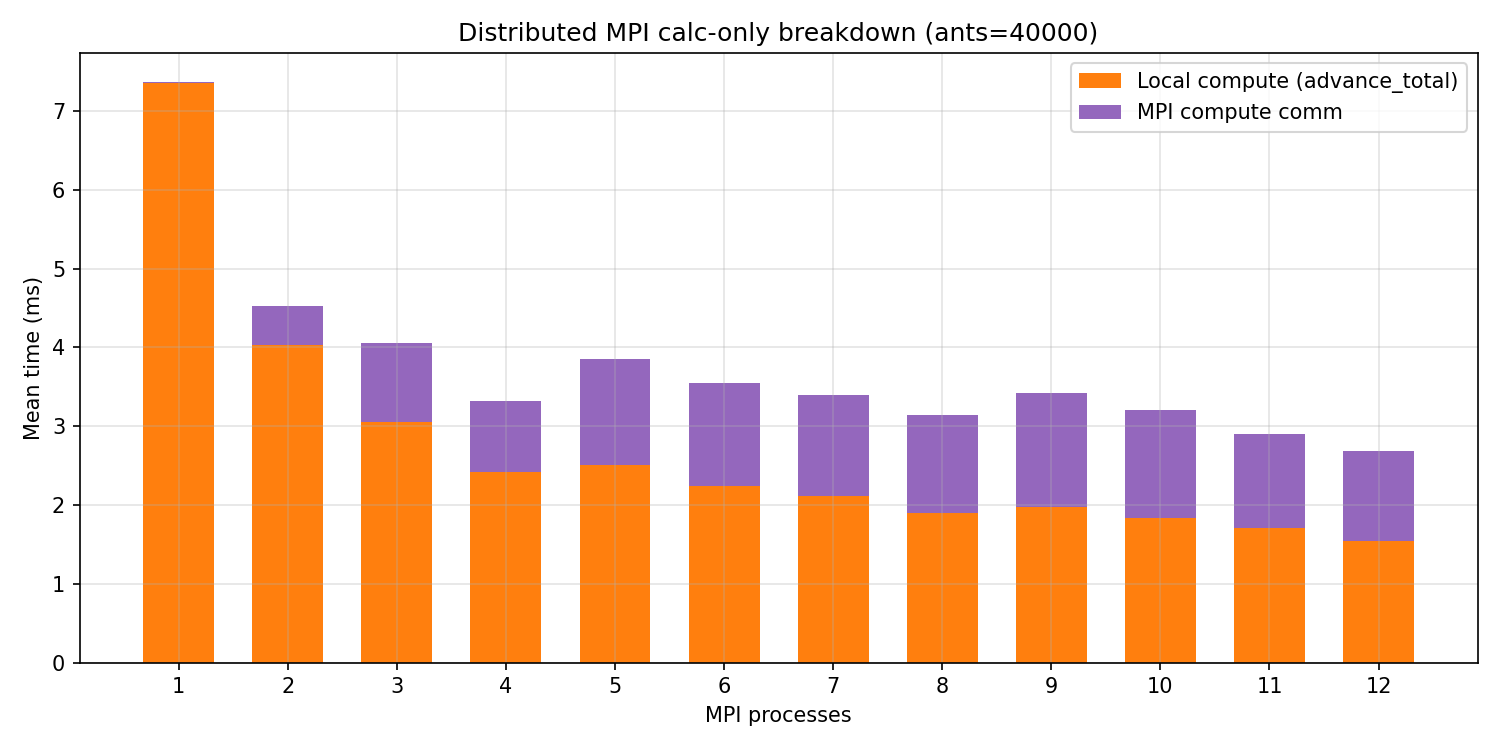
\includegraphics[width=\linewidth]{../distributed_subdomain_mpi/results/sweeps_render_food10/plots/mpi_calc_only_ants40000.png}
    \\[-2mm]
    {\footnotesize (b) 40000 ants}
\end{minipage}

\vspace{1mm}
\begin{minipage}{0.62\columnwidth}
    \centering
    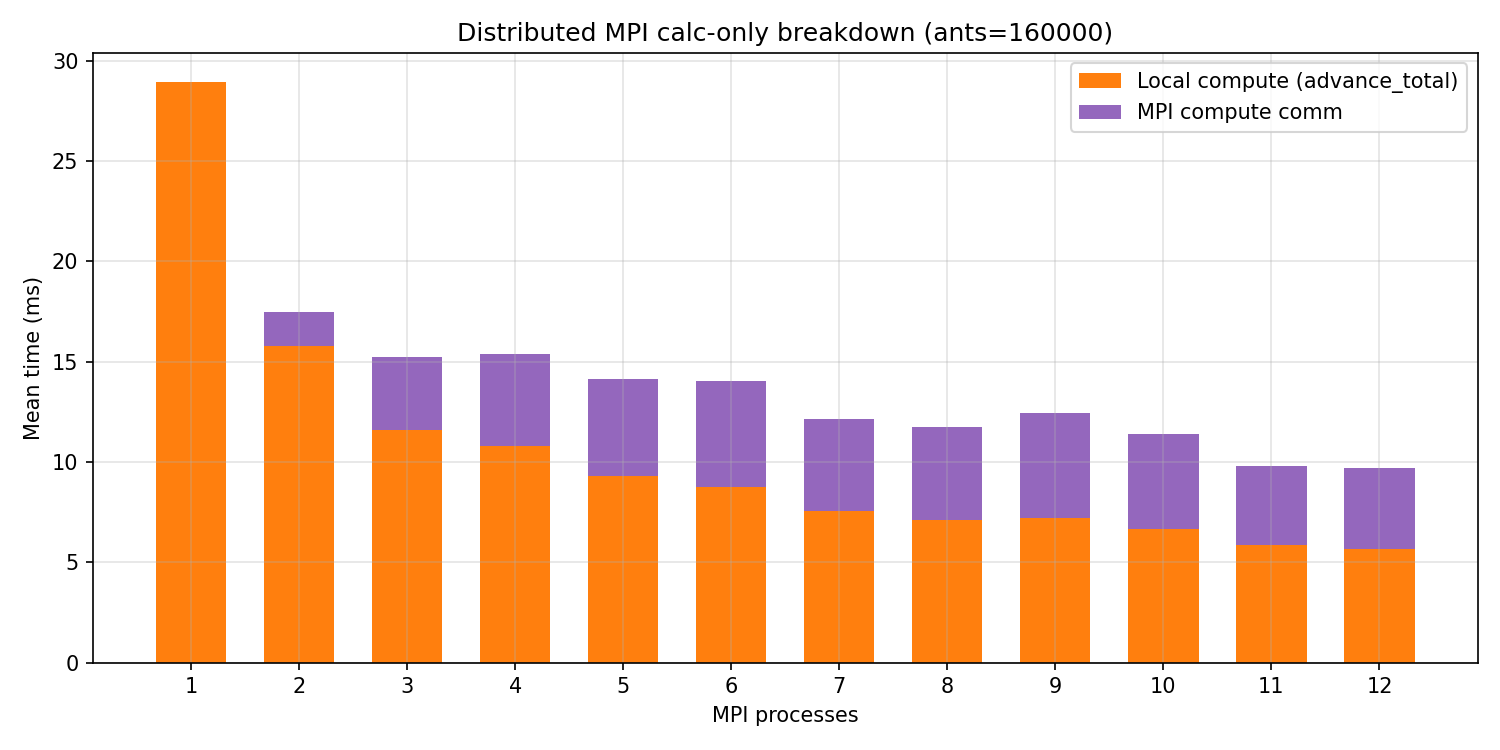
\includegraphics[width=\linewidth]{../distributed_subdomain_mpi/results/sweeps_render_food10/plots/mpi_calc_only_ants160000.png}
    \\[-2mm]
    {\footnotesize (c) 160000 ants}
\end{minipage}
\caption{MPI subdomain computation-only breakdown for selected colony sizes.}
\label{fig:mpi_calc_only_selected}
\end{figure}
% Auto-generated. Do not edit by hand.
\begin{table}[!htbp]
\centering
\caption{MPI compute speedup for all colony sizes and MPI process counts.}
\label{tab:mpi_speedup}
\normalsize
\setlength{\tabcolsep}{2.4pt}
\renewcommand{\arraystretch}{1.08}
\begin{tabular}{lcccccc}
\toprule
\textbf{Proc/Ants} & \textbf{5k} & \textbf{10k} & \textbf{20k} & \textbf{40k} & \textbf{80k} & \textbf{160k} \\
\midrule
1 & 1.00 & 1.00 & 1.00 & 1.00 & 1.00 & 1.00 \\
2 & 1.52 & 1.52 & 2.01 & 1.63 & 1.69 & 1.66 \\
3 & 1.72 & 1.80 & 1.94 & 1.82 & 1.84 & 1.90 \\
4 & 2.00 & 1.87 & 2.67 & 2.22 & 2.42 & 1.88 \\
5 & 1.58 & 1.54 & 2.14 & 1.91 & 1.96 & 2.05 \\
6 & 2.38 & 1.60 & 2.44 & 2.07 & 2.06 & 2.06 \\
7 & 1.87 & 1.76 & 2.70 & 2.17 & 2.41 & 2.38 \\
8 & 1.87 & 1.76 & 2.70 & 2.34 & 2.42 & 2.46 \\
9 & 1.73 & 1.80 & 2.61 & 2.16 & 2.35 & 2.32 \\
10 & 1.76 & 1.90 & 2.83 & 2.30 & 2.49 & 2.54 \\
11 & 1.81 & 2.11 & 3.05 & 2.54 & 2.78 & 2.96 \\
12 & 1.96 & 2.23 & 3.07 & 2.75 & 2.86 & 2.99 \\
\bottomrule
\end{tabular}
\par\vspace{2pt}\parbox{\columnwidth}{\raggedright\footnotesize\textit{Note.} The compute metric is $advance\_total + mpi\_halo\_exchange + mpi\_migration + mpi\_food\_allreduce$, matching the MPI compute plots. Efficiency is computed with respect to the number of compute MPI processes only; rendering is excluded from the process count. For each colony size, the baseline is the smallest available MPI process count $p_0$. Each cell reports speedup $S=T(p_0)/T(p)$.}
\end{table}

% Auto-generated. Do not edit by hand.
\begin{table}[!htbp]
\centering
\caption{MPI compute efficiency for all colony sizes and MPI process counts.}
\label{tab:mpi_efficiency}
\normalsize
\setlength{\tabcolsep}{2.4pt}
\renewcommand{\arraystretch}{1.08}
\begin{tabular}{lcccccc}
\toprule
\textbf{Proc/Ants} & \textbf{5k} & \textbf{10k} & \textbf{20k} & \textbf{40k} & \textbf{80k} & \textbf{160k} \\
\midrule
1 & 1.00 & 1.00 & 1.00 & 1.00 & 1.00 & 1.00 \\
2 & 0.76 & 0.76 & 1.01 & 0.81 & 0.85 & 0.83 \\
3 & 0.57 & 0.60 & 0.65 & 0.61 & 0.61 & 0.63 \\
4 & 0.50 & 0.47 & 0.67 & 0.55 & 0.61 & 0.47 \\
5 & 0.32 & 0.31 & 0.43 & 0.38 & 0.39 & 0.41 \\
6 & 0.40 & 0.27 & 0.41 & 0.35 & 0.34 & 0.34 \\
7 & 0.27 & 0.25 & 0.39 & 0.31 & 0.34 & 0.34 \\
8 & 0.23 & 0.22 & 0.34 & 0.29 & 0.30 & 0.31 \\
9 & 0.19 & 0.20 & 0.29 & 0.24 & 0.26 & 0.26 \\
10 & 0.18 & 0.19 & 0.28 & 0.23 & 0.25 & 0.25 \\
11 & 0.16 & 0.19 & 0.28 & 0.23 & 0.25 & 0.27 \\
12 & 0.16 & 0.19 & 0.26 & 0.23 & 0.24 & 0.25 \\
\bottomrule
\end{tabular}
\par\vspace{2pt}\parbox{\columnwidth}{\raggedright\footnotesize\textit{Note.} The compute metric is $advance\_total + mpi\_halo\_exchange + mpi\_migration + mpi\_food\_allreduce$, matching the MPI compute plots. Efficiency is computed with respect to the number of compute MPI processes only; rendering is excluded from the process count. For each colony size, the baseline is the smallest available MPI process count $p_0$. Each cell reports efficiency $E=S/(p/p_0)$.}
\end{table}


Nevertheless, it is evident that, unlike the case of parallelization with shared memory, there is an improvement in performance with the incorporation of processes which, although conditioned by the size of the buffers in which information is stored and also by the cost of communications, means that from the incorporation of more than one computation thread onward, the MPI parallelization shows, over the vast majority of the domain, a better performance per iteration than the OpenMP parallelization, as can be seen in Fig.~\ref{fig:mpi_vs_omp_calc_selected}.

For a direct three-way comparison between OMP-only, MPI-only, and Hybrid MPI+OMP sweeps, the script \texttt{docs/scripts/plot\_compare\_omp\_mpi\_hybrid.py} generates the figures under \texttt{docs/figures/compare\_omp\_mpi\_hybrid/}.

\begin{figure}[!htbp]
\centering
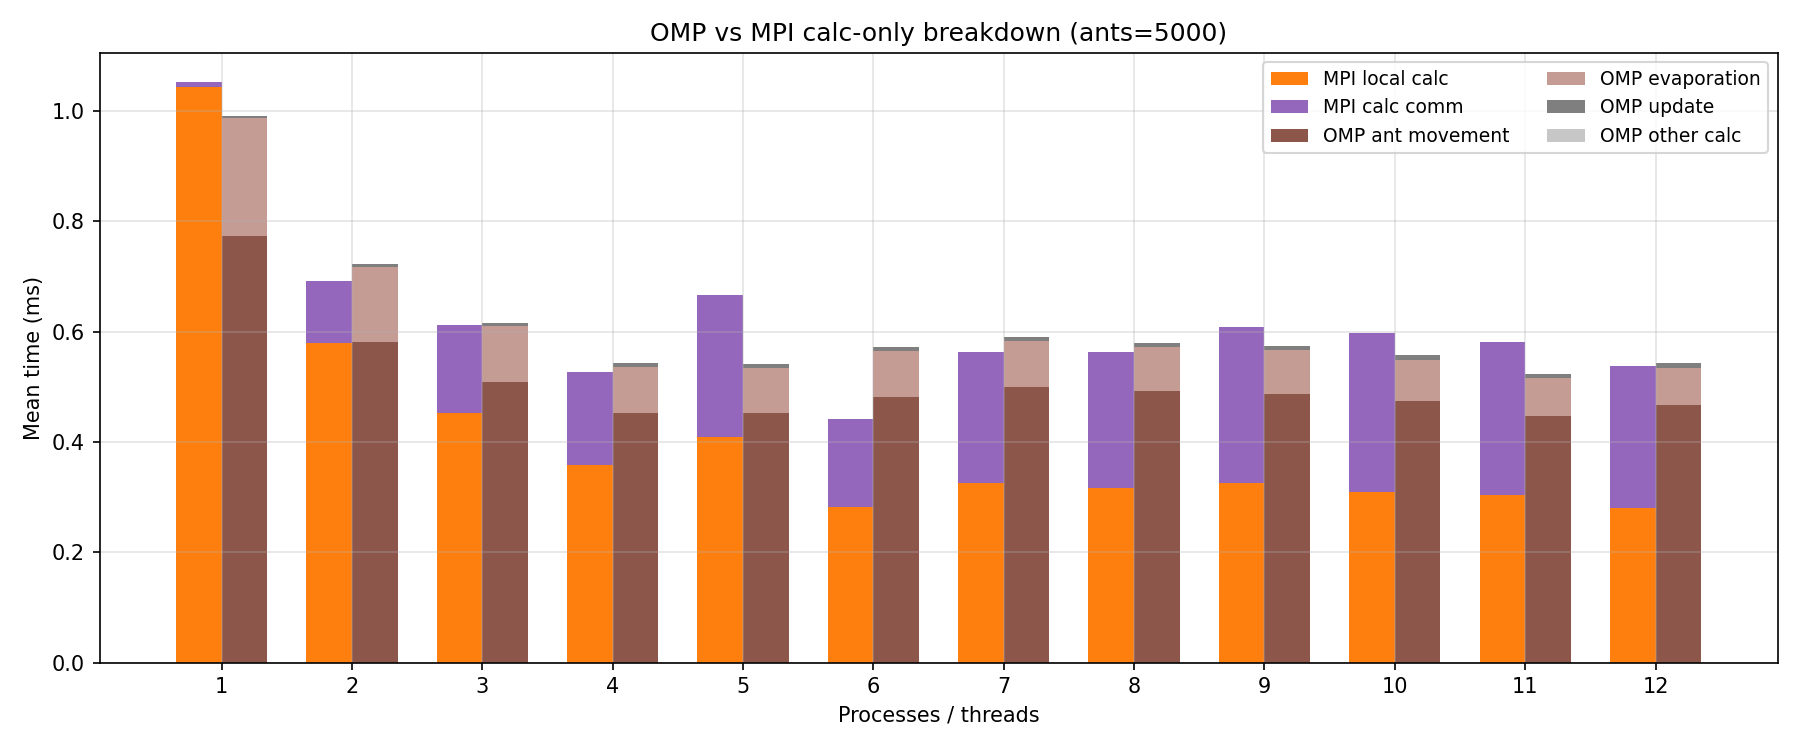
\includegraphics[width=0.90\columnwidth]{figures/compare_subdomain_omp/compare_calc_ants5000.png}
\\[-2mm]
{\footnotesize (a) 5000 ants}
\vspace{1mm}
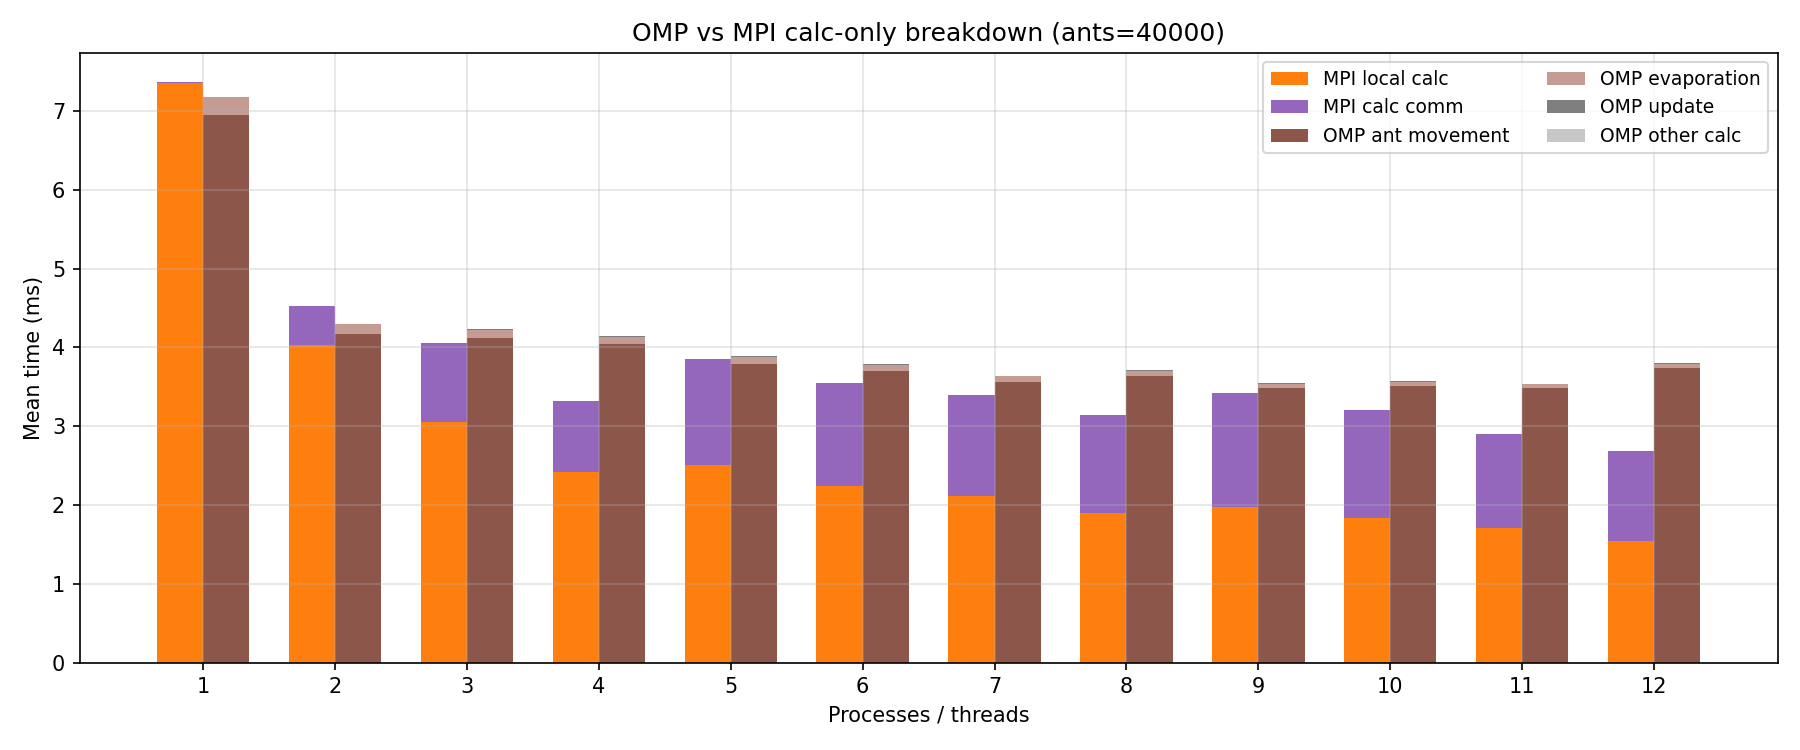
\includegraphics[width=0.90\columnwidth]{figures/compare_subdomain_omp/compare_calc_ants40000.png}
\\[-2mm]
{\footnotesize (b) 40000 ants}
\vspace{1mm}
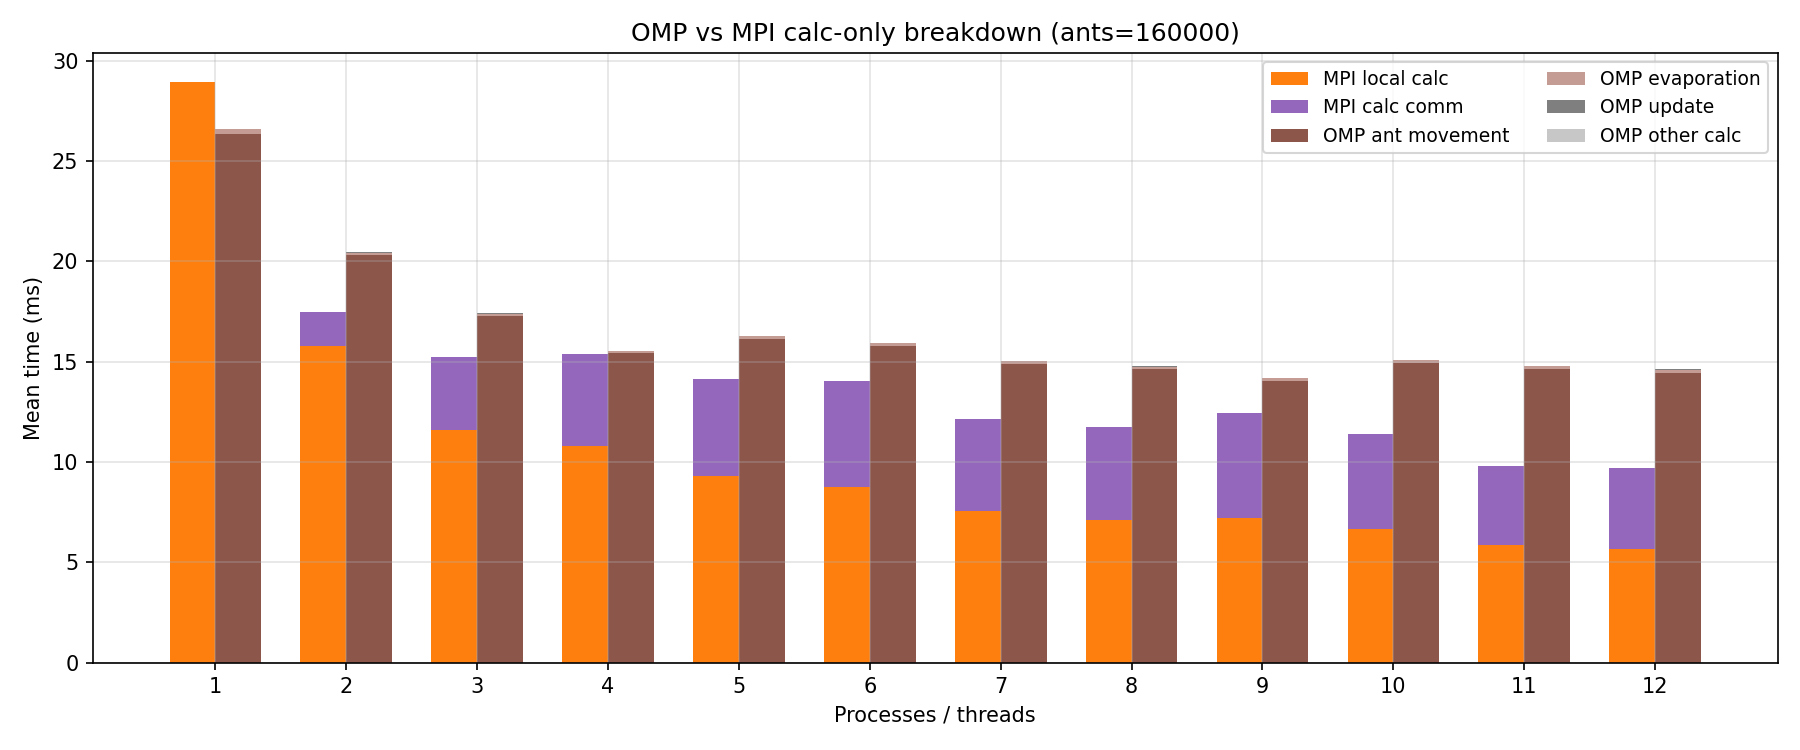
\includegraphics[width=0.90\columnwidth]{figures/compare_subdomain_omp/compare_calc_ants160000.png}
\\[-2mm]
{\footnotesize (c) 160000 ants}
\caption{MPI subdomain vs OpenMP computation-only breakdown for selected colony sizes.}
\label{fig:mpi_vs_omp_calc_selected}
\end{figure}

A relevant conclusion is that as has been discused the scaling of the subdomain strategy is jointly limited by communication growth and memory-traffic pressure in migration buffers as the process count and colony size increase. Consequently, although the inclusion of more processes improves performance over a broad operating region, the incremental gain per added process decreases at high process counts, which is consistent with the observed separation between the speedup with communication and the speedup without communication.

\subsection{Hybrid distributed subdomain}
Considering the particularities of the solution implemented over the subdomains, the implementation of a hybrid model for the ant colonies is proposed, given that the cost of increasing the number of subdomains using MPI parallelization became evident, but it also became evident that the increase in subdomains causes a considerable increase in the number of communication operations between subdomains. Within this framework, hybrid integration is proposed as a solution so that each one of the subdomains has threads that execute in parallel with shared memory using OpenMP, as contrasted in Fig.~\ref{fig:hybrid_compare_calc_selected}. The objective is not necessarily to reengineer the algorithm, but rather to integrate shared-memory threads within each subdomain in order to increase parallelism in the computation without incurring the already mentioned costly communication costs associated with an increase in the number of subdomains into which the fractal terrain is decomposed.

\begin{figure}[!t]
\centering
\begin{minipage}{0.48\columnwidth}
    \centering
    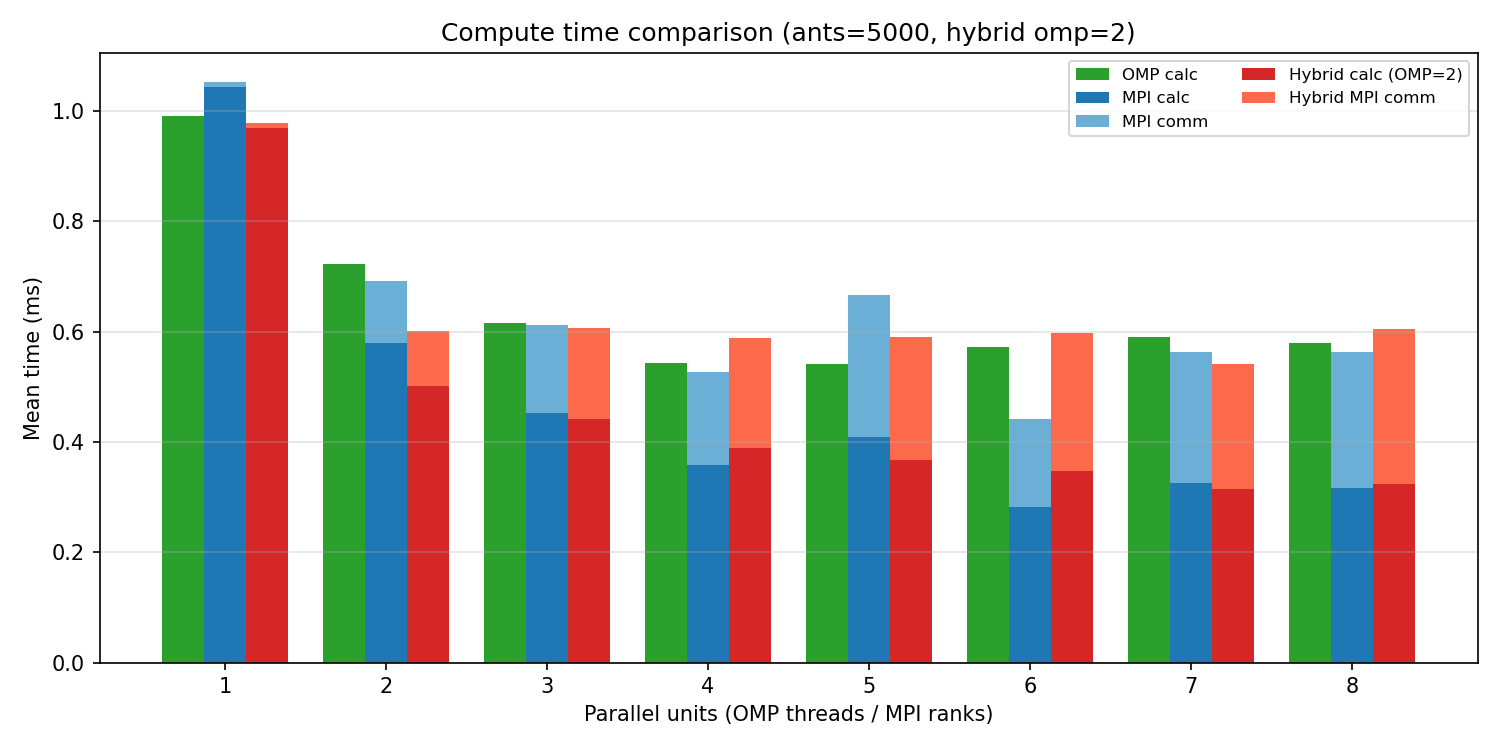
\includegraphics[width=\linewidth]{figures/compare_omp_mpi_hybrid/compare3_calc_omp2_ants5000.png}
    \\[-2mm]
    {\footnotesize (a) OMP=2, 5000 ants}
\end{minipage}
\hfill
\begin{minipage}{0.48\columnwidth}
    \centering
    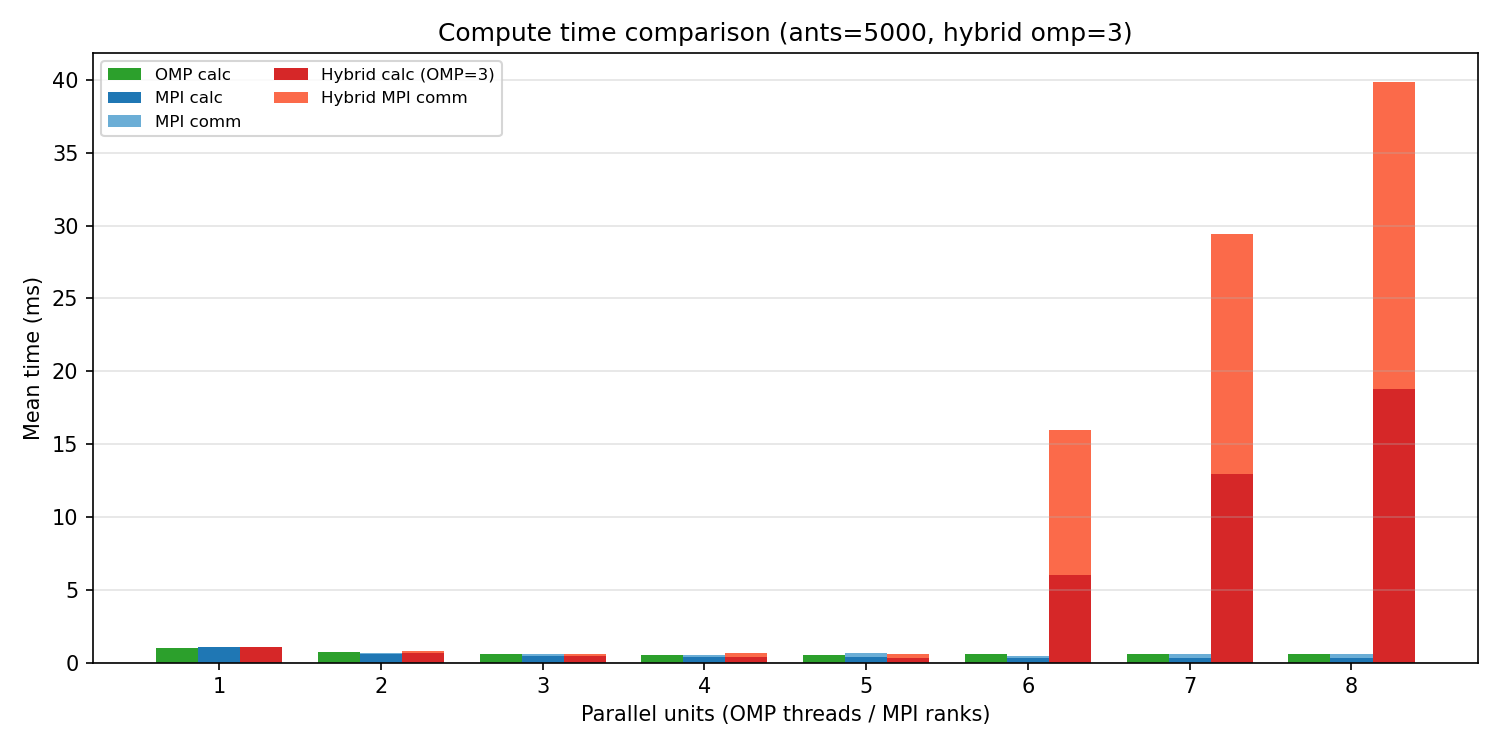
\includegraphics[width=\linewidth]{figures/compare_omp_mpi_hybrid/compare3_calc_omp3_ants5000.png}
    \\[-2mm]
    {\footnotesize (b) OMP=3, 5000 ants}
\end{minipage}

\vspace{1mm}
\begin{minipage}{0.48\columnwidth}
    \centering
    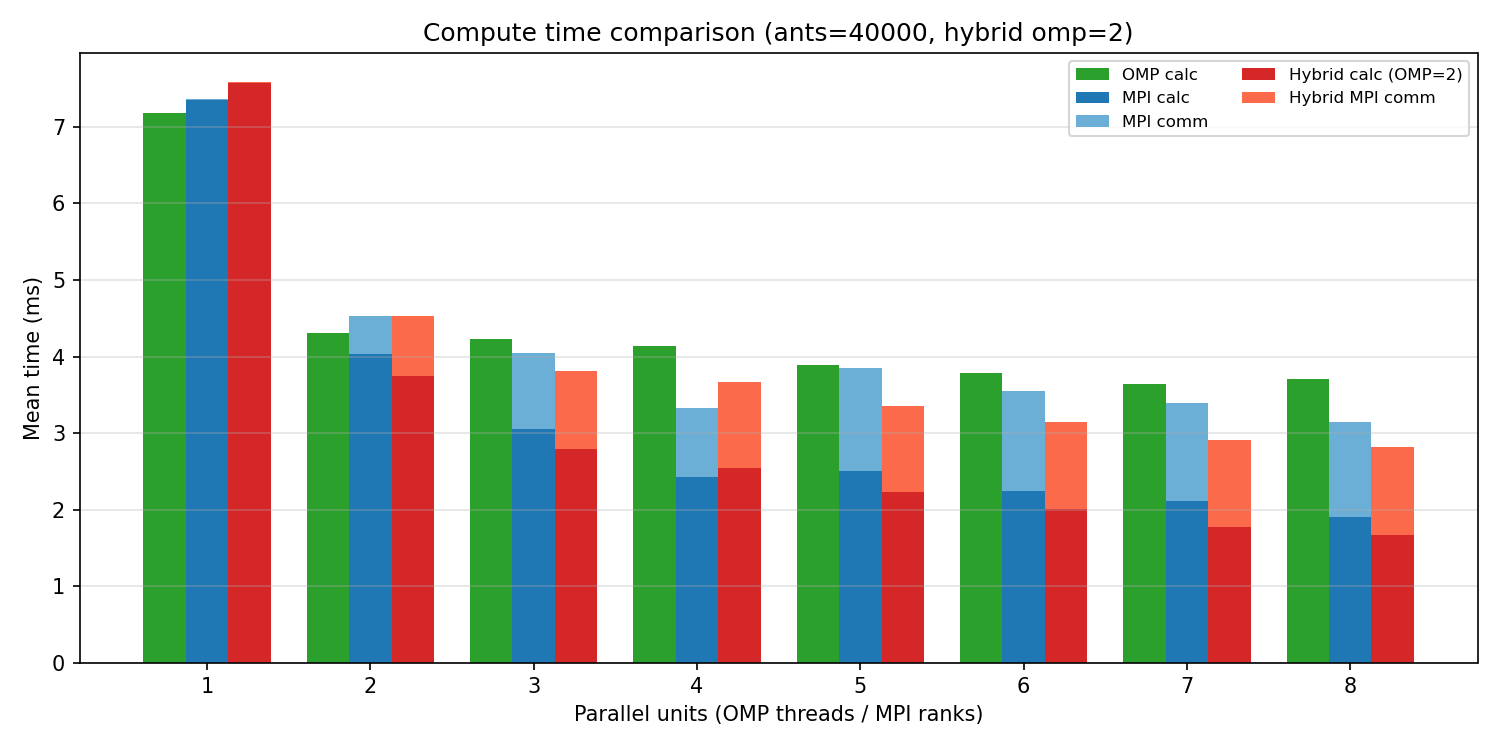
\includegraphics[width=\linewidth]{figures/compare_omp_mpi_hybrid/compare3_calc_omp2_ants40000.png}
    \\[-2mm]
    {\footnotesize (c) OMP=2, 40000 ants}
\end{minipage}
\hfill
\begin{minipage}{0.48\columnwidth}
    \centering
    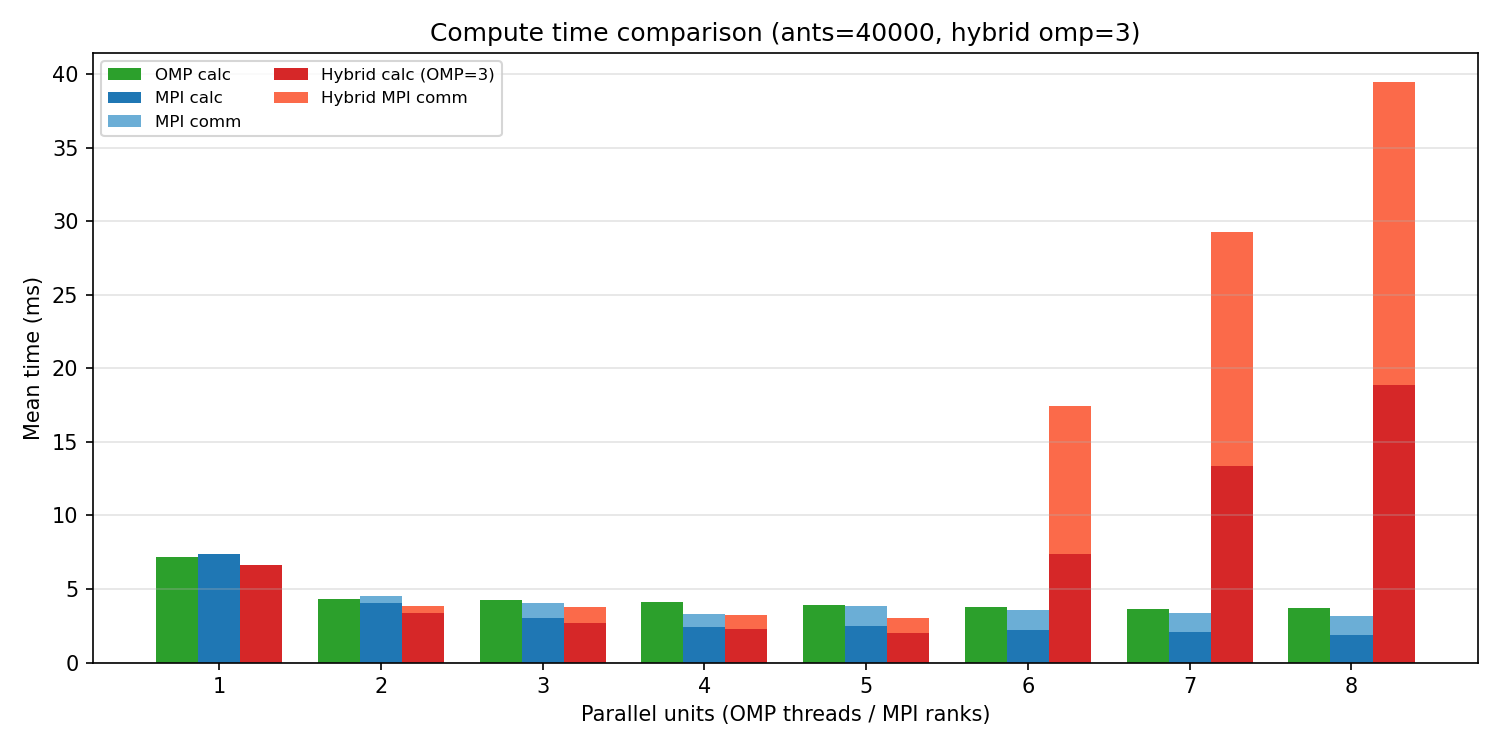
\includegraphics[width=\linewidth]{figures/compare_omp_mpi_hybrid/compare3_calc_omp3_ants40000.png}
    \\[-2mm]
    {\footnotesize (d) OMP=3, 40000 ants}
\end{minipage}

\vspace{1mm}
\begin{minipage}{0.48\columnwidth}
    \centering
    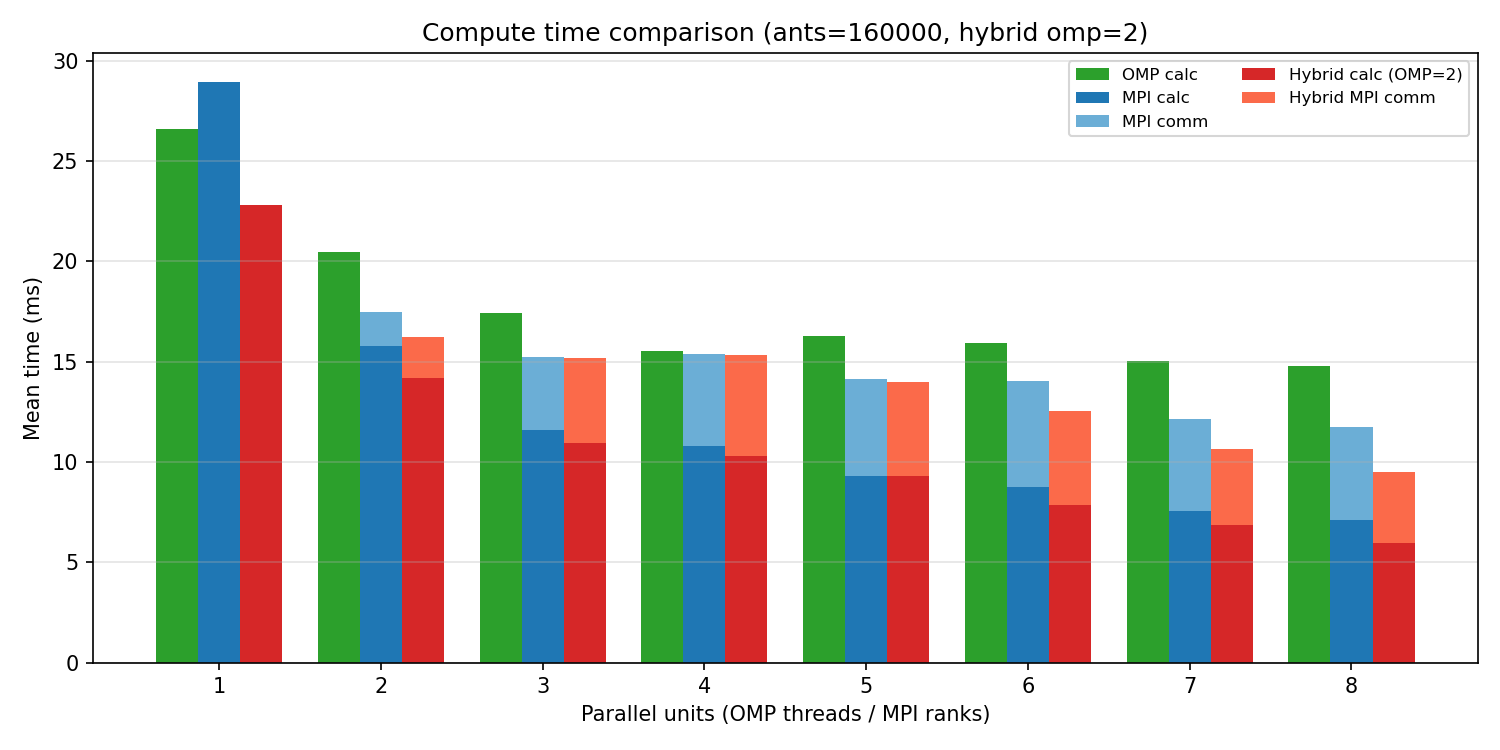
\includegraphics[width=\linewidth]{figures/compare_omp_mpi_hybrid/compare3_calc_omp2_ants160000.png}
    \\[-2mm]
    {\footnotesize (e) OMP=2, 160000 ants}
\end{minipage}
\hfill
\begin{minipage}{0.48\columnwidth}
    \centering
    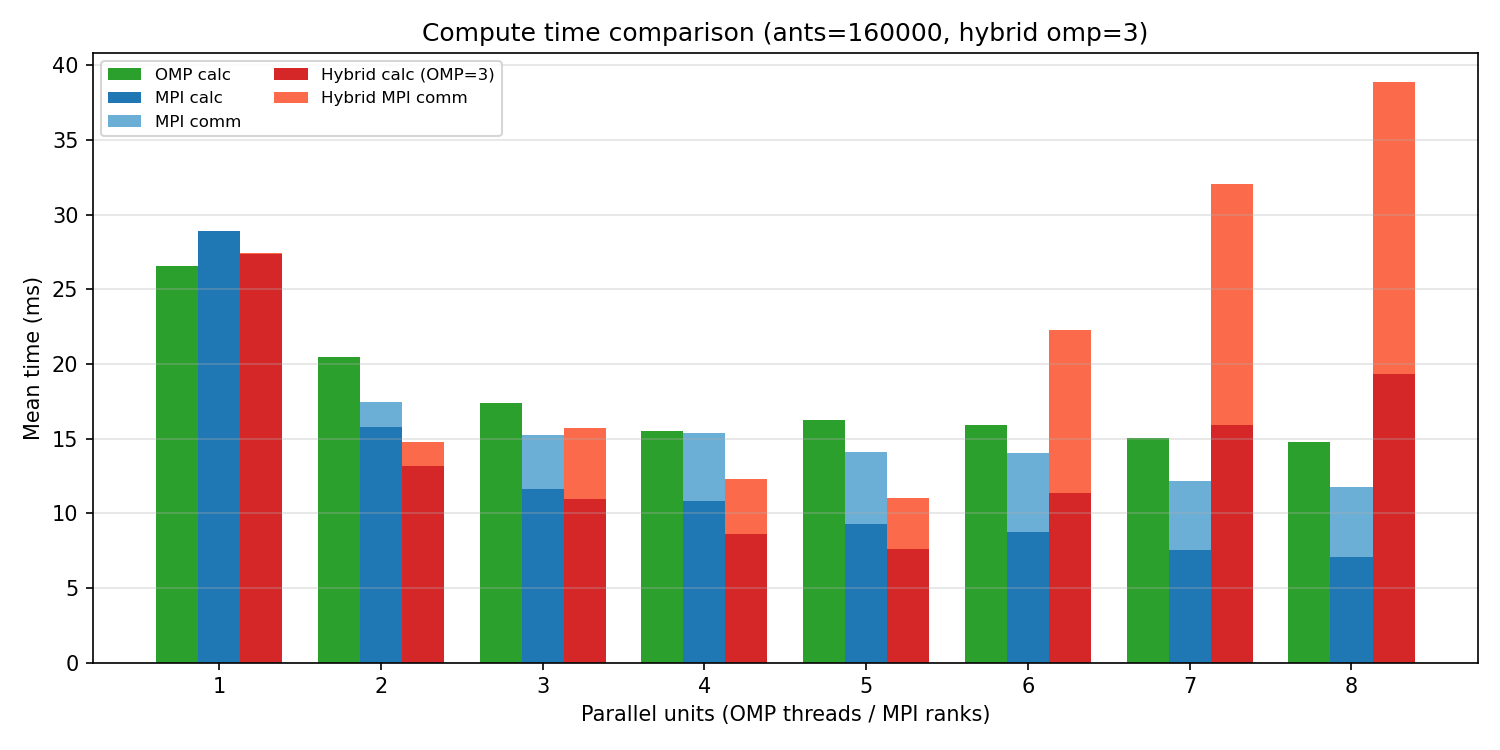
\includegraphics[width=\linewidth]{figures/compare_omp_mpi_hybrid/compare3_calc_omp3_ants160000.png}
    \\[-2mm]
    {\footnotesize (f) OMP=3, 160000 ants}
\end{minipage}
\caption{Hybrid OMP-only vs MPI-only vs MPI+OpenMP computation-only comparison for selected colony sizes. The left column corresponds to two OpenMP threads per subdomain and the right column corresponds to three OpenMP threads per subdomain. The associated efficiency is computed with respect to compute MPI processes only, excluding rendering.}
\label{fig:hybrid_compare_calc_selected}
\end{figure}
% Auto-generated. Do not edit by hand.
\begin{table}[!htbp]
\centering
\caption{Hybrid MPI+OpenMP compute speedup for OMP=2 threads per rank.}
\label{tab:hybrid_speedup_omp2}
\normalsize
\setlength{\tabcolsep}{2.4pt}
\renewcommand{\arraystretch}{1.08}
\begin{tabular}{lcccccc}
\toprule
\textbf{Proc/Ants} & \textbf{5k} & \textbf{10k} & \textbf{20k} & \textbf{40k} & \textbf{80k} & \textbf{160k} \\
\midrule
1 & 1.00 & 1.00 & 1.00 & 1.00 & 1.00 & 1.00 \\
2 & 1.63 & 1.44 & 1.47 & 1.68 & 1.74 & 1.41 \\
3 & 1.61 & 1.50 & 1.71 & 1.99 & 1.60 & 1.50 \\
4 & 1.66 & 1.50 & 1.76 & 2.07 & 1.79 & 1.49 \\
5 & 1.66 & 1.55 & 1.93 & 2.26 & 1.78 & 1.63 \\
6 & 1.64 & 1.69 & 1.74 & 2.41 & 2.02 & 1.82 \\
7 & 1.81 & 1.89 & 1.89 & 2.61 & 2.47 & 2.14 \\
8 & 1.62 & 1.91 & 2.06 & 2.69 & 2.03 & 2.40 \\
\bottomrule
\end{tabular}
\par\vspace{2pt}\parbox{\columnwidth}{\raggedright\footnotesize\textit{Note.} The compute metric is $advance\_total + mpi\_halo\_exchange + mpi\_migration + mpi\_food\_allreduce$, matching the hybrid sweep plots. Efficiency is computed with respect to the number of compute MPI processes only; rendering is excluded from the process count. For each combination of colony size and OpenMP threads per rank, the baseline is the smallest available MPI process count $p_0$. Each cell reports speedup $S=T(p_0)/T(p)$.}
\end{table}

% Auto-generated. Do not edit by hand.
\begin{table}[!htbp]
\centering
\caption{Hybrid MPI+OpenMP compute efficiency for OMP=2 threads per rank.}
\label{tab:hybrid_efficiency_omp2}
\normalsize
\setlength{\tabcolsep}{2.4pt}
\renewcommand{\arraystretch}{1.08}
\begin{tabular}{lcccccc}
\toprule
\textbf{Proc/Ants} & \textbf{5k} & \textbf{10k} & \textbf{20k} & \textbf{40k} & \textbf{80k} & \textbf{160k} \\
\midrule
1 & 1.00 & 1.00 & 1.00 & 1.00 & 1.00 & 1.00 \\
2 & 0.81 & 0.72 & 0.74 & 0.84 & 0.87 & 0.70 \\
3 & 0.54 & 0.50 & 0.57 & 0.66 & 0.53 & 0.50 \\
4 & 0.42 & 0.38 & 0.44 & 0.52 & 0.45 & 0.37 \\
5 & 0.33 & 0.31 & 0.39 & 0.45 & 0.36 & 0.33 \\
6 & 0.27 & 0.28 & 0.29 & 0.40 & 0.34 & 0.30 \\
7 & 0.26 & 0.27 & 0.27 & 0.37 & 0.35 & 0.31 \\
8 & 0.20 & 0.24 & 0.26 & 0.34 & 0.25 & 0.30 \\
\bottomrule
\end{tabular}
\par\vspace{2pt}\parbox{\columnwidth}{\raggedright\footnotesize\textit{Note.} The compute metric is $advance\_total + mpi\_halo\_exchange + mpi\_migration + mpi\_food\_allreduce$, matching the hybrid sweep plots. Efficiency is computed with respect to the number of compute MPI processes only; rendering is excluded from the process count. For each combination of colony size and OpenMP threads per rank, the baseline is the smallest available MPI process count $p_0$. Each cell reports efficiency $E=S/(p/p_0)$.}
\end{table}

% Auto-generated. Do not edit by hand.
\begin{table}[!htbp]
\centering
\caption{Hybrid MPI+OpenMP compute speedup for OMP=3 threads per rank.}
\label{tab:hybrid_speedup_omp3}
\normalsize
\setlength{\tabcolsep}{2.4pt}
\renewcommand{\arraystretch}{1.08}
\begin{tabular}{lcccccc}
\toprule
\textbf{Proc/Ants} & \textbf{5k} & \textbf{10k} & \textbf{20k} & \textbf{40k} & \textbf{80k} & \textbf{160k} \\
\midrule
1 & 1.00 & 1.00 & 1.00 & 1.00 & 1.00 & 1.00 \\
2 & 1.37 & 1.27 & 1.70 & 1.72 & 1.68 & 1.85 \\
3 & 1.79 & 1.83 & 2.01 & 1.77 & 1.96 & 1.74 \\
4 & 1.69 & 1.58 & 2.02 & 2.06 & 2.21 & 2.23 \\
5 & 1.92 & 1.76 & 2.48 & 2.20 & 2.30 & 2.48 \\
6 & 0.07 & 0.12 & 0.23 & 0.38 & 0.76 & 1.23 \\
7 & 0.04 & 0.07 & 0.12 & 0.23 & 0.44 & 0.85 \\
8 & 0.03 & 0.05 & 0.10 & 0.17 & 0.34 & 0.70 \\
\bottomrule
\end{tabular}
\par\vspace{2pt}\parbox{\columnwidth}{\raggedright\footnotesize\textit{Note.} The compute metric is $advance\_total + mpi\_halo\_exchange + mpi\_migration + mpi\_food\_allreduce$, matching the hybrid sweep plots. Efficiency is computed with respect to the number of compute MPI processes only; rendering is excluded from the process count. For each combination of colony size and OpenMP threads per rank, the baseline is the smallest available MPI process count $p_0$. Each cell reports speedup $S=T(p_0)/T(p)$.}
\end{table}

% Auto-generated. Do not edit by hand.
\begin{table}[!htbp]
\centering
\caption{Hybrid MPI+OpenMP compute efficiency for OMP=3 threads per rank.}
\label{tab:hybrid_efficiency_omp3}
\normalsize
\setlength{\tabcolsep}{2.4pt}
\renewcommand{\arraystretch}{1.08}
\begin{tabular}{lcccccc}
\toprule
\textbf{Proc/Ants} & \textbf{5k} & \textbf{10k} & \textbf{20k} & \textbf{40k} & \textbf{80k} & \textbf{160k} \\
\midrule
1 & 1.00 & 1.00 & 1.00 & 1.00 & 1.00 & 1.00 \\
2 & 0.69 & 0.64 & 0.85 & 0.86 & 0.84 & 0.93 \\
3 & 0.60 & 0.61 & 0.67 & 0.59 & 0.65 & 0.58 \\
4 & 0.42 & 0.40 & 0.51 & 0.51 & 0.55 & 0.56 \\
5 & 0.38 & 0.35 & 0.50 & 0.44 & 0.46 & 0.50 \\
6 & 0.01 & 0.02 & 0.04 & 0.06 & 0.13 & 0.20 \\
7 & 0.01 & 0.01 & 0.02 & 0.03 & 0.06 & 0.12 \\
8 & 0.00 & 0.01 & 0.01 & 0.02 & 0.04 & 0.09 \\
\bottomrule
\end{tabular}
\par\vspace{2pt}\parbox{\columnwidth}{\raggedright\footnotesize\textit{Note.} The compute metric is $advance\_total + mpi\_halo\_exchange + mpi\_migration + mpi\_food\_allreduce$, matching the hybrid sweep plots. Efficiency is computed with respect to the number of compute MPI processes only; rendering is excluded from the process count. For each combination of colony size and OpenMP threads per rank, the baseline is the smallest available MPI process count $p_0$. Each cell reports efficiency $E=S/(p/p_0)$.}
\end{table}

% Auto-generated. Do not edit by hand.
\begin{table}[!htbp]
\centering
\caption{Hybrid MPI+OpenMP compute speedup for OMP=4 threads per rank.}
\label{tab:hybrid_speedup_omp4}
\normalsize
\setlength{\tabcolsep}{2.4pt}
\renewcommand{\arraystretch}{1.08}
\begin{tabular}{lcccccc}
\toprule
\textbf{Proc/Ants} & \textbf{5k} & \textbf{10k} & \textbf{20k} & \textbf{40k} & \textbf{80k} & \textbf{160k} \\
\midrule
1 & 1.00 & 1.00 & 1.00 & 1.00 & 1.00 & 1.00 \\
2 & 1.41 & 1.45 & 1.78 & 1.70 & 1.59 & 1.84 \\
3 & 1.68 & 1.73 & 1.77 & 1.83 & 1.49 & 1.85 \\
4 & 1.86 & 1.72 & 2.15 & 2.04 & 2.10 & 2.25 \\
5 & 0.04 & 0.07 & 0.14 & 0.26 & 0.44 & 0.83 \\
6 & 0.03 & 0.05 & 0.09 & 0.17 & 0.31 & 0.66 \\
7 & 0.03 & 0.04 & 0.09 & 0.16 & 0.28 & 0.59 \\
8 & 0.02 & 0.03 & 0.05 & 0.09 & 0.17 & 0.36 \\
\bottomrule
\end{tabular}
\par\vspace{2pt}\parbox{\columnwidth}{\raggedright\footnotesize\textit{Note.} The compute metric is $advance\_total + mpi\_halo\_exchange + mpi\_migration + mpi\_food\_allreduce$, matching the hybrid sweep plots. Efficiency is computed with respect to the number of compute MPI processes only; rendering is excluded from the process count. For each combination of colony size and OpenMP threads per rank, the baseline is the smallest available MPI process count $p_0$. Each cell reports speedup $S=T(p_0)/T(p)$.}
\end{table}

% Auto-generated. Do not edit by hand.
\begin{table}[!htbp]
\centering
\caption{Hybrid MPI+OpenMP compute efficiency for OMP=4 threads per rank.}
\label{tab:hybrid_efficiency_omp4}
\normalsize
\setlength{\tabcolsep}{2.4pt}
\renewcommand{\arraystretch}{1.08}
\begin{tabular}{lcccccc}
\toprule
\textbf{Proc/Ants} & \textbf{5k} & \textbf{10k} & \textbf{20k} & \textbf{40k} & \textbf{80k} & \textbf{160k} \\
\midrule
1 & 1.00 & 1.00 & 1.00 & 1.00 & 1.00 & 1.00 \\
2 & 0.71 & 0.73 & 0.89 & 0.85 & 0.80 & 0.92 \\
3 & 0.56 & 0.58 & 0.59 & 0.61 & 0.50 & 0.62 \\
4 & 0.47 & 0.43 & 0.54 & 0.51 & 0.52 & 0.56 \\
5 & 0.01 & 0.01 & 0.03 & 0.05 & 0.09 & 0.17 \\
6 & 0.00 & 0.01 & 0.02 & 0.03 & 0.05 & 0.11 \\
7 & 0.00 & 0.01 & 0.01 & 0.02 & 0.04 & 0.08 \\
8 & 0.00 & 0.00 & 0.01 & 0.01 & 0.02 & 0.04 \\
\bottomrule
\end{tabular}
\par\vspace{2pt}\parbox{\columnwidth}{\raggedright\footnotesize\textit{Note.} The compute metric is $advance\_total + mpi\_halo\_exchange + mpi\_migration + mpi\_food\_allreduce$, matching the hybrid sweep plots. Efficiency is computed with respect to the number of compute MPI processes only; rendering is excluded from the process count. For each combination of colony size and OpenMP threads per rank, the baseline is the smallest available MPI process count $p_0$. Each cell reports efficiency $E=S/(p/p_0)$.}
\end{table}


From the results of the hybrid implementation, it becomes evident that when two threads are implemented for each process, the computation execution-time results improve according to the number of processes, in most cases even more when the number of ants is larger and the increase in the parallel computing units favors the reduction of computation time. When the loads are medium or large, however, it is still evident that the fragmentation of the domain continues to cause significant increases in the time associated with migration, which means that although the computation time improves, the improvement is not sufficiently significant with respect to MPI parallelization when the total computation time is considered, as can be seen in the results for two threads per subdomain, which is the number of threads per subdomain that showed the best result in the test simulations.

It is also worth highlighting that when the number of MPI processes is increased and, in addition, the number of threads per rank is increased, each thread receives very few ants and the cost of coordinating those threads begins to consume an important part of the computation time, as can be seen in Fig.~\ref{fig:hybrid_compare_calc_selected}. For this reason, in the implementation of the hybrid model, too many threads per process become inefficient when the local subdomain is no longer sufficiently large, because the useful work per thread is not sufficiently significant and the cost of coordination and distribution of the results grows disproportionately with respect to the performance gain that it provides in the computation.

\clearpage

\begin{thebibliography}{00}
\bibitem{Dorigo} M. Dorigo, V. Maniezzo, and A. Colorni, ``Ant system: Optimization by a colony of cooperating agents,'' \textit{IEEE Transactions on Systems, Man, and Cybernetics---Part B: Cybernetics}, vol. 26, no. 1, pp. 29--41, Feb. 1996.
\end{thebibliography}
\end{document}
